%==============================================================
% Part 1 : The introduction 
%==============================================================
% \let\rbackup\r
% \newcommand{\x}{{\mathbf{x}}}
% \renewcommand{\u}{{\mathbf{u}}}
% \newcommand{\w}{\mathbf{w}}
% \newcommand{\y}{{\mathbf{y}}}
% \newcommand{\bx}{\x}
% \newcommand{\bu}{\u}
% \newcommand{\bv}{v}
% \newcommand{\btau}{\tau}
% \newcommand{\by}{{\tilde\y}}
% \newcommandx{\xb}[2][1=n,2=k]{\x_{#1|#2}}
% \newcommandx{\ub}[2][1=n,2=k]{\u_{#1|#2}}
% \newcommandx{\wb}[2][1=n,2=k]{\w_{#1|#2}}
% \renewcommand{\r}{\mathbf{r}}
% \newcommand{\rx}{\r^\x}
% \newcommand{\ru}{\r^\u}
% \newcommand{\vv}{{{v}}}
% \newcommandx{\gb}[3][1=n,2=k,3={}]{g_{#1|#2}^{#3}}
% \newcommandx{\hb}[3][1=n,2=k,3={}]{h_{#1}^{#3}}
% \newcommandx{\vb}[2][1=n,2=k]{\vv_{#1|#2}}
% \newcommandx{\tb}[2][1=n,2=k]{\tau_{#1|#2}}
% \newcommand{\blambda}{{\boldsymbol{\lambda}}}
% \newcommand{\bmu}{{\boldsymbol{\mu}}}
% \newcommand{\rr}{{\mathrm{r}}}
% \newcommand{\ff}{\mathrm{f}}
% \newcommand{\bxi}{{\boldsymbol{\xi}}}
% \newcommand{\bet}{{\boldsymbol{\nu}}}
% \newcommand{\ped}{\mathrm{ped}}
% \newcommand{\rped}{\r^\ped}
% \newcommand{\rxped}{\r^{\x,\ped}}
% \newcommand{\ruped}{\r^{\u,\ped}}

% \newcommand{\matr}[2]{\left[\begin{array}{#1}#2\end{array}\right]}

% !TEX root=../../Thesis.tex
\chapter{Introduction} \label{ch:intro}
The way we transport ourselves is currently evolving, and \gls{ad} technology is expected to have a big impact on this transformation~\cite{traffic21, McKinsey2023}. With \gls{av} the efficiency of traffic can be improved by scheduling commercial transports outside of rush hours~\cite{FAGNANT2015167}. Number of parking spots in cities can be reduced if the vehicles can autonomously drive itself to a less crowded area when not in use and drive back when needed. Congestion and traffic jams could also be reduced if a large amount of vehicles in traffic are autonomous and optimize around the same goal e.g., traffic flow or fuel efficiency. 

The rapid success of \gls{ml} during the last decades has lead to major progress towards deploying \gls{av}s in the real world. One clear benefactor of these new \gls{ml} technics are the perception systems~\cite{Janai2020}. Better perception enables more accurate representation of the environment. 
% The low-level control of the vehicle is a mature research area and can be solved with classical control theory methods~\cite{Paden2016}.
However, navigating complex scenarios such as urban intersections and roundabouts with dense traffic remain challenging for \gls{av}s because it requires a higher level of interaction between road users, as summarized in a review paper~\cite{Schwarting2018}. 
When a human driver approach an intersection, they observe the environment to identify the traffic light, signs and other approaching vehicles. Then assess the situation to determine \textit{who has the right of way?} Before deciding weather to drive or yield. 
% If all drivers could perfectly assess the situation and follow the right of way, there would be no accidents or collisions between cars. 
% Despite, each year over one million people are killed in traffic-related accidents, where the vast majority of the accidents are caused by human mistakes~\cite{WHO2018, NHTSA2018}. 
But human drivers are not perfect, according to the Insurance Institute for Highway Safety~\cite{IIHS2019}, in 2019, an estimated \num{115741} people were injured by drivers running a red light, whereas \num{928} of them were killed. 
While these accidents were mainly caused by driver inattention or reckless driving, it motivates the development of decision-making algorithms for \gls{av}s which not only follow the traffic rules but can also take into account other drivers future actions and inattention, which is the main focus in this thesis. 
%\todo{Level 2: Volvo pilot assist and tesla auto pilot. Level 4: Waymo. Woven automated city}
% That is why this thesis will focus on intersection scenarios that includes interactions of other vehicles and propose a \gls{rl} approach using deep Q-learning while considering the uncertainty of . 

% This thesis presents a deep Q-learning approach for creating decision-making strategies for \gls{av}s driving in environments with other drivers without explicitly knowing their intentions. 
% Starting with introducing the different \gls{ad} levels in Section~\ref{sec:intro_ad}.
% Section~\ref{sec:intro_intersections} defines the terms' scenario, intersection and intention used in this thesis.
% \Citet{Shalev2016} raises two concerns when using \gls{ml}, especially Reinforcement learning, for autonomous driving applications: ensuring functional safety of the driving policy and solving the \gls{mdp} model is problematic, because of unpredictable behavior of other drivers. 
% Ensuring functional safety is not the main focus of this work, but because of its importance, it is briefly addressed in Section~\ref{sec:system_architecture} together with a proposed system architecture that can utilize the work presented in this thesis in a ''safe'' way. 
% The handling of the unpredictable behavior of other drivers is the main topic in this thesis and the research questions are presented in Section~\ref{sec:research_questions}. The scope and limitations are listed in Section~\ref{sec:scope}. Finally, the contributions of this thesis is presented in Section~\ref{sec:contributions}. 

\section{Autonomous Driving Levels}
\label{sec:intro_ad}
When talking about autonomous driving, it is first important to specify which level of autonomy that is being discussed. The Society of Automotive Engineers has classified these different levels of autonomy ranging from zero to five~\cite{SAE2021}, also referred to as L0-L5. The first level L0 is a vehicle with no autonomy, whereas a fully \gls{av} that can operate in any environment and without any human supervision is defined as L5. Popular \gls{adas} functions today, like lane centering or adaptive cruise control are classified as L1, while the Volvo Pilot Assist and Tesla Autopilot that provide both steering and acceleration/breaking are classified as level 2. The main criteria for L2 systems is that the driver is in control and only supported by the system. This puts a requirement on the driver to always supervise the vehicle and take over when needed to ensure safety. For L3 and higher the responsibility of driving is shifted to the system. At L3, the driver still has to take control over the vehicle but at only the request of the system, and at L4 and L5 the autonomous driving features no longer require the driver to take over. Finally, the main difference between L4 and L5 is the capability of driving anywhere, under all conditions. Examples of L4 are robot taxis developed by Waymo, Zoox, cruise and Toyota which only operate in a specified area or city. 

% Another way to categorize these autonomy levels is: supervised and unsupervised driving. Supervised driving include L0-L3 where the driver has to supervise the system and take control when necessary, while unsupervised 
% \tommy{Level 2: You are diving, provide steering and breaking support to the driver, lane centering and adaptive cruise control}

The \gls{av} making the decisions in this work are referred to as the ego vehicle, while other traffic participants are assumed to be vehicles driven by other human drivers but could be extended to pedestrians bicyclist and other \gls{av}s. 
The methods presented in this thesis are aimed at an autonomy level L5. At this level the system is expected to handle all aspects of driving within a specific task such as crossing an intersection. 


\section{Intersections, intention and scenarios}
\label{sec:intro_intersections}
When it comes to the scenarios considered in this work. This section aims to clarify the use of the words' intersection, intention and scenario.
% When a pedestrian approach a crossing they have been taught at a young age to look at both sides of the road before crossing. The same apply for a human driver approaching an intersection. 
% When a human driver approach an intersection, it is natural to observe the environment to identify the traffic light, signs and other approaching vehicles. Then assess the situation, who has the right of way? 

% The intention of the other driver can be guided by the 
% Recently nontraditional intersections are also becoming increasingly popular. The goal of these designs is to reduce the number and/or severity of conflict points by altering the customary vehicular paths at the intersection. In light of the increased focus on and occurrence of these intersection types, it is expected that the application of nontraditional designs will continue to spread.

\begin{figure}[h]
	\centering
	\begin{subfigure}[t]{0.48\columnwidth}
		\centering
		\begin{tikzpicture}
			% Crossing
			\def\crossleftx{-2}
			\def\crossrightx{2}
			\def\crosstopy{2}
			\def\crossboty{-2}
			\def\roadwidth{0.5}

			\draw (0,0) circle (2pt);
			\node at (1.2, 0.2) {conflict point};
			\draw[thick] (\crossleftx, \roadwidth) -- (-\roadwidth, \roadwidth) -- (-\roadwidth, \crosstopy);
			\draw[thick] (\crossleftx, -\roadwidth) -- (-\roadwidth, -\roadwidth) -- (-\roadwidth-\roadwidth, \crossboty);
			\draw[thick] (\roadwidth, \crosstopy) -- (\roadwidth, \roadwidth) -- (\crossrightx, \roadwidth);
			\draw[thick] (\roadwidth-\roadwidth, \crossboty) -- (\roadwidth, -\roadwidth) -- (\crossrightx, -\roadwidth);

			% 	cars
			\node[inner sep=0pt] (ego_car) at (\crossleftx+0.5,0)
			{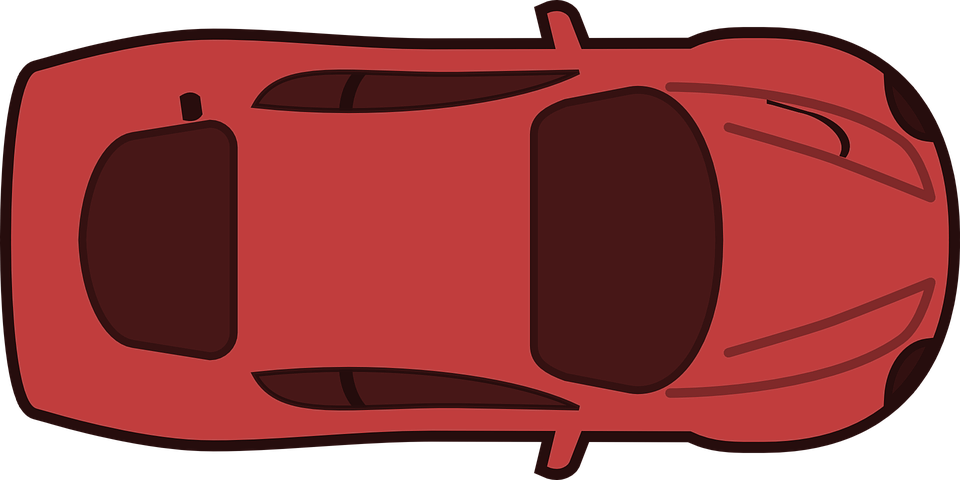
\includegraphics[width=.18\textwidth, angle=0]{figures/ego_car_top_down.png}};

			\node[inner sep=0pt] (target_car) at (0,\crosstopy-0.5)
			{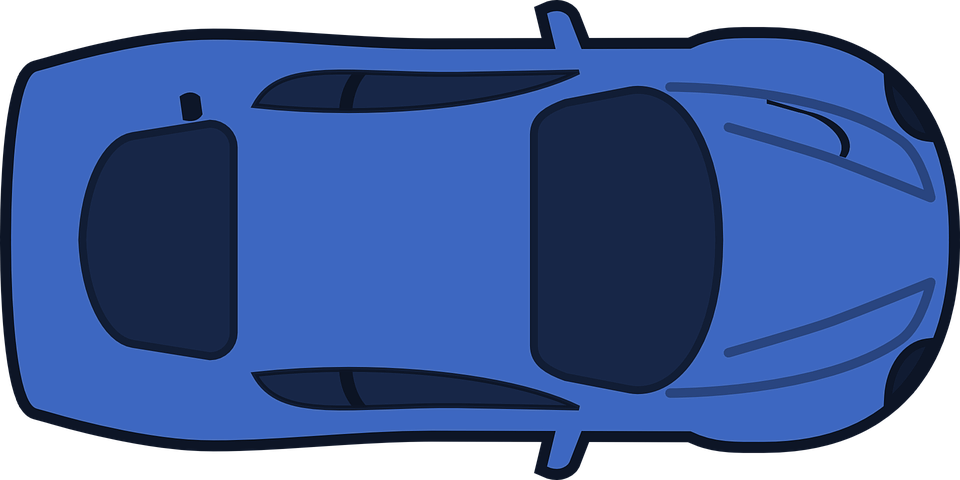
\includegraphics[width=.18\textwidth, angle=-90]{figures/target_car_top_down.png}};

			\node[inner sep=0pt] (target_car) at (-.1,-0.8)
			{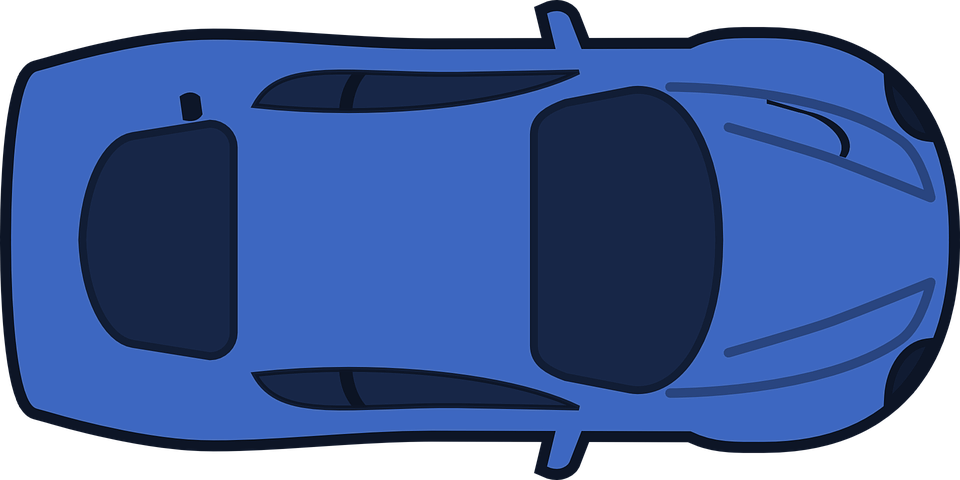
\includegraphics[width=.18\textwidth, angle=-110]{figures/target_car_top_down.png}};


		\end{tikzpicture}
		\caption{Single intersection}
\end{subfigure}%
	~ 
	\begin{subfigure}[t]{0.48\columnwidth}
		\centering
		\begin{tikzpicture}
			% Crossing
			\def\crossleftx{-2.5}
			\def\crossrightx{2.5}
			\def\crosstopy{2}
			\def\crossboty{-2}
			\def\roadwidth{0.5}

			\draw (-0.5,0) circle (2pt);
			\draw (0.5,0) circle (2pt);
			% \node at (0.7, 0.2) {crossing point$^1$};
			\draw[thick] (\crossleftx, \roadwidth) -- (-\roadwidth-0.5, \roadwidth) -- (-\roadwidth-0.5, \crosstopy);
			\draw[thick] (\crossleftx, -\roadwidth) -- (-\roadwidth-0.5, -\roadwidth) -- (-\roadwidth-0.5, \crossboty);
			\draw[thick] (0, \crosstopy) -- (0, \roadwidth);
			\draw[thick] (0, -\roadwidth) -- (0, \crossboty);
			\draw[thick] (\roadwidth+0.5, \crosstopy) -- (\roadwidth+0.5, \roadwidth) -- (\crossrightx, \roadwidth);
			\draw[thick] (\roadwidth+0.5, \crossboty) -- (\roadwidth+0.5, -\roadwidth) -- (\crossrightx, -\roadwidth);

			% 	cars
			\node[inner sep=0pt] (ego_car) at (\crossleftx+0.5,0)
			{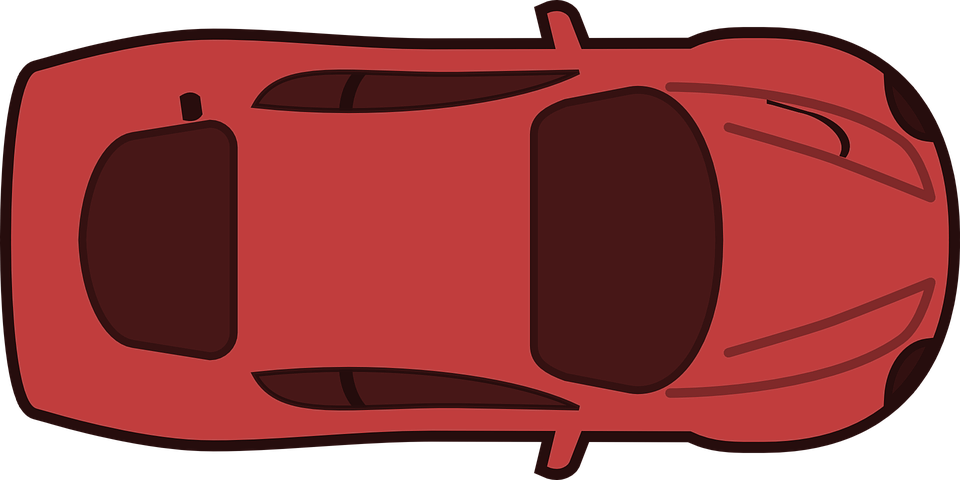
\includegraphics[width=.18\textwidth, angle=0]{figures/ego_car_top_down.png}};

			\node[inner sep=0pt] (target_car) at (-0.5,\crosstopy-0.5) {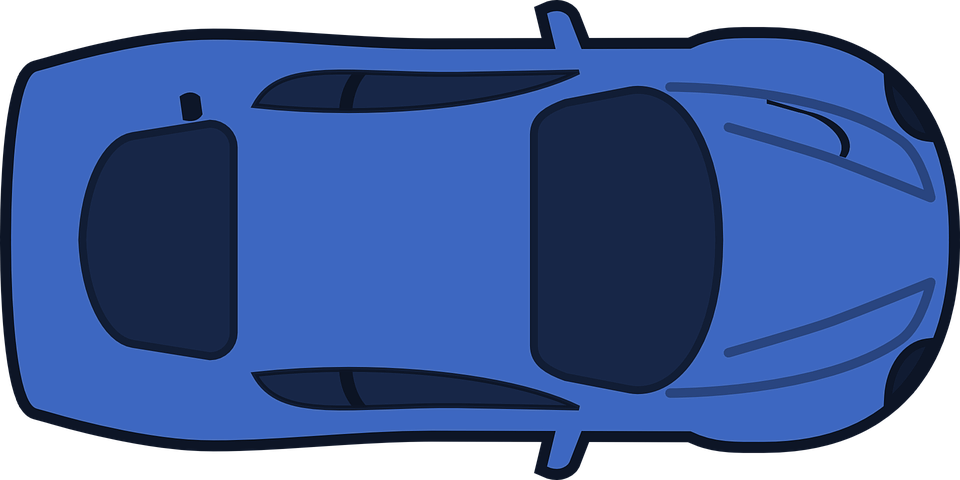
\includegraphics[width=.18\textwidth, angle=-90]{figures/target_car_top_down.png}};

			\node[inner sep=0pt] (target_car_2) at (0.5,\crossboty+0.5) {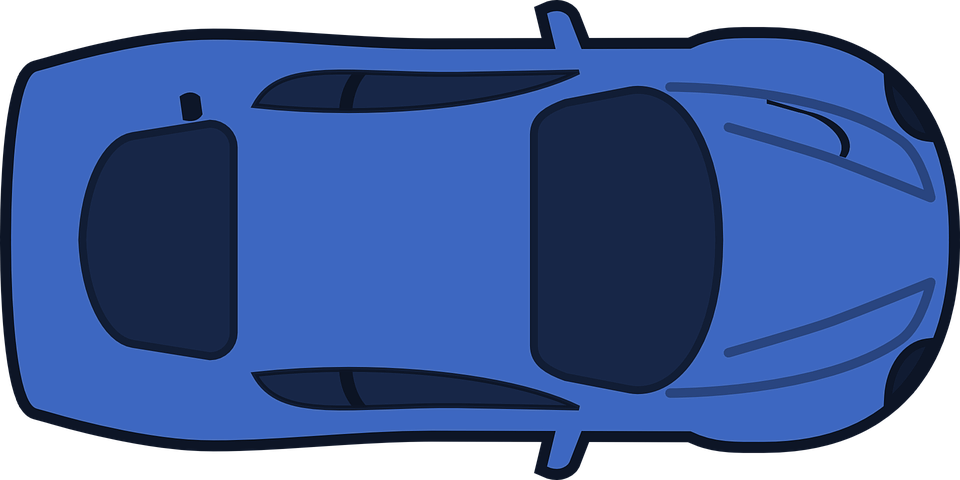
\includegraphics[width=.18\textwidth, angle=90]{figures/target_car_top_down.png}};

		\end{tikzpicture}
		\caption{Double intersection}
	\end{subfigure}

	\caption{Examples of different intersections}
	\label{fig:example_intersections}
\end{figure}
Let's begin by defining the terms 'intersection,' 'intention,' and 'scenario' within the context of this study.
An intersection refers to the geometric layout of roads intersecting each other, encompassing elements such as the number of junctions, conflict points, turns, and angles of incidence, as illustrated in Figure~\ref{fig:example_intersections}. 
Intersections can be categorized as signalized or unsignalized. A signalized intersection is equipped with mechanisms to designate the right-of-way, such as regulatory signs (e.g., STOP or YIELD) or traffic signals, while an unsignalized intersection lacks such features. However, as emphasized in the introduction, human drivers do not always adhere strictly to these right-of-way rules, which can result in accidents. Therefore, this thesis defines intentions as the anticipated actions of other vehicles in the future, such as stopping, cautiously slowing down, or proceeding through the intersection.

\begin{figure}[h]
	% \mbox{\parbox{\textwidth}{
	% \centering
	% % \vspace{0.3cm}
	% 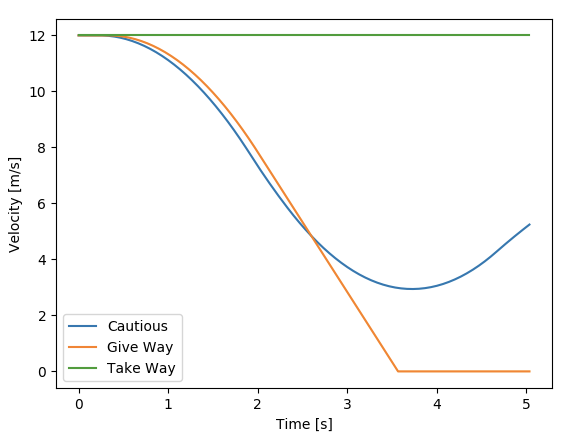
\includegraphics[width=0.6\columnwidth]{YourThesis/papers/mpc/figures/velocity_profiles_agents.png}
	% }}
	\centering
	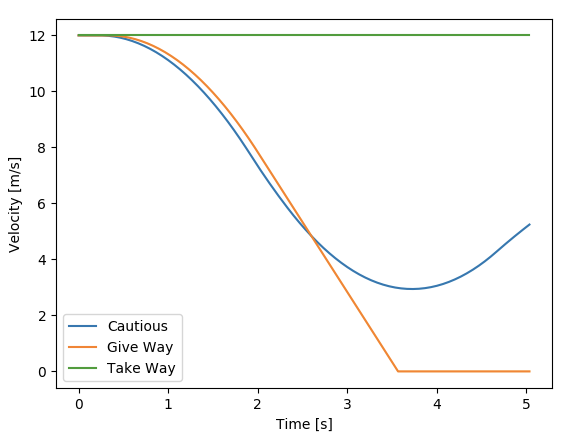
\includegraphics[width=0.6\columnwidth]{YourThesis/papers/mpc/figures/velocity_profiles_agents.png}

	\caption{An illustration showing velocity profiles for agents with three distinct intentions. Each agent shares the same initial position and velocity while approaching a common intersection.}
	\label{fig:intro_intention_profiles}
	% \vspace{-0.3cm}
\end{figure}

Figure \ref{fig:intro_intention_profiles} illustrates how velocity profiles can differ for three different intentions. In this example, distinguishing between the 'give way' and 'take way' intentions is straightforward, as the velocity begins to decelerate at time $0$. However, identifying the 'cautious' intention poses a challenge, as the agent cannot be certain until the other vehicle comes to a complete stop.

If intentions are known, intersections can be treated as unsignalized, as the right-of-way can be inferred from the intentions rather than relying solely on infrastructure. This approach ensures safety even in situations where another vehicle disregards traffic rules, such as running a red light, as a cautious agent will prioritize safety and stop accordingly.

\section{The intersection problem}
\begin{figure}
	\mbox{\parbox{\textwidth}{
		\centering
		\begin{tikzpicture}
			\def\xstart{-7};

			\coordinate (p) at (3,0);
			\foreach \n/\w/\c in {z0/2/green,z1/2/red,z2/2.5/orange,z3/3.5/blue}{
				\node[rectangle,
				draw=none,
				anchor=east,
				text = black,
				fill = \c!60,
				minimum width = \w cm, 
				minimum height = 2cm] 
				(n) at (p) {\Huge \n};
				
				\coordinate (p) at (n.west);
			}

			% Crossing
			\draw[line width=0.5mm] (\xstart, 1) -- (-1, 1) -- (-1, 5);
			\draw[line width=0.5mm] (\xstart, -1) -- (-1, -1) -- (-1, -2);
			\draw[line width=0.5mm] (1, 5) -- (1, 1) -- (3, 1);
			\draw[line width=0.5mm] (1, -2) -- (1, -1) -- (3, -1);
			
			% cars
			\node[inner sep=0pt] (ego_car) at (-7,0)
			{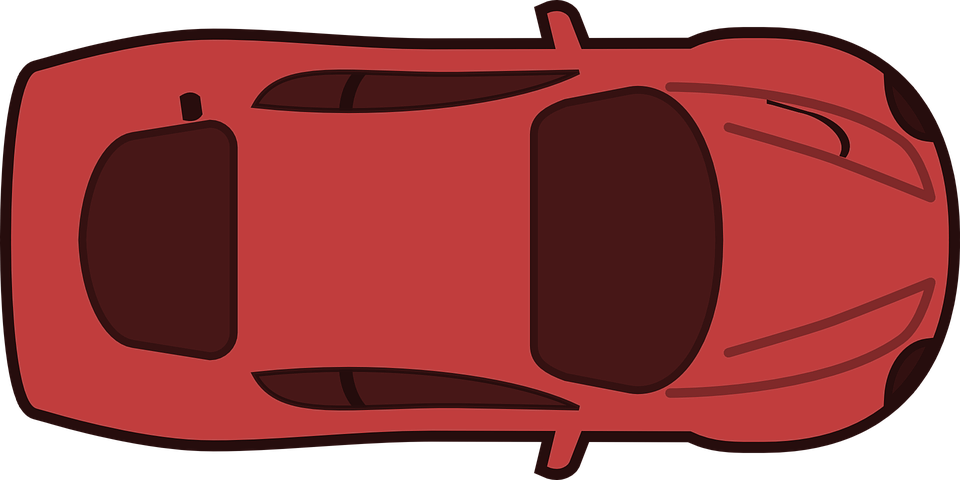
\includegraphics[width=.18\textwidth, angle=0]{figures/ego_car_top_down.png}};
			\node[inner sep=0pt] (target_car) at (0,4)
			{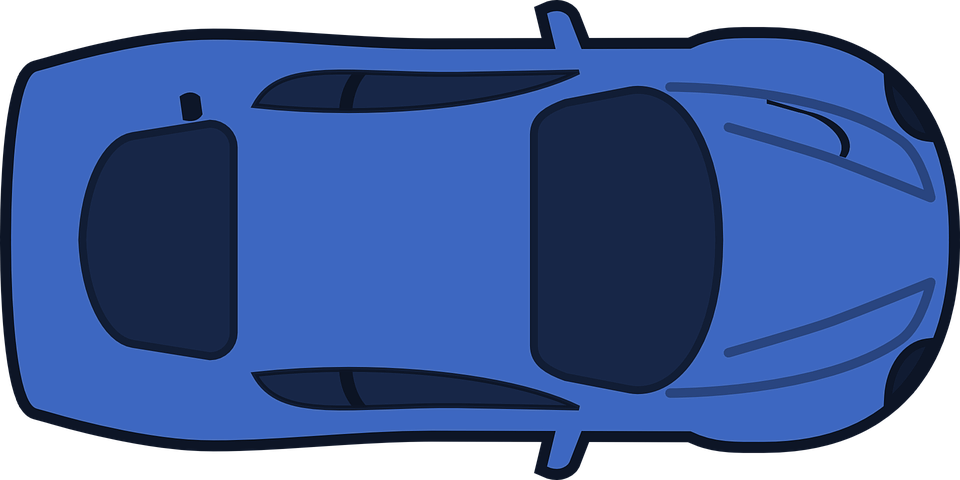
\includegraphics[width=.18\textwidth, angle=-90]{figures/target_car_top_down.png}};

	\end{tikzpicture}
	}}
	\caption{Intersection scenario divided into zones describing what is required of the decision maker in different zones}
	\label{fig:zones}
\end{figure}

With the \gls{mdp} defined, the path of the ego vehicle can be segmented into four zones as shown in Figure~\ref{fig:zones}. Starting from the end, Zone 0 represents the 'safe zone,' where the ego vehicle is out of danger and can resume nominal driving. Zone 1 is the 'conflict zone,' where a collision with another vehicle is possible. Zone 2, the 'critical decision zone,' is the final opportunity for the vehicle to either stop or proceed through the intersection. The size of zone 2 is determined by the minimum distance required for the vehicle to come to a complete stop before entering the conflict zone, ensuring sufficient time for safe decision-making. Lastly, Zone 3, the 'information gathering zone,' is situated furthest from the intersection. Here, the agent can observe how other vehicles behave over time to estimate their intentions.

The goal is to reach Zone 0. To achieve this, the agent aims to minimize the time spent in Zone 1 if there is a chance of intersection with another car. Our actions are formulated as short-term goals, designed for comfortable use with lower acceleration rates. The size of Zone 2 depends on the vehicle's current speed, which is influenced by its behavior in Zone 3.

Now, two conflicting strategies emerge: to minimize time in Zone 1, the agent desires a high speed entering the intersection. However, it also seeks a low speed to reduce the size of Zone 2 and the critical decision period. If the intentions of other vehicles are known, the stochasticity in Zone 1 would be eliminated, transforming the problem into a scheduling task aimed at creating a velocity profile that minimizes the time required to cross. However, since the intentions of other vehicles are stochastic, reinforcement learning offers a promising approach to address this uncertainty and optimize decision-making in dynamic traffic scenarios.



\section{Research questions}
\label{sec:research_questions}
% This thesis defines human driving as sequential decision making under uncertainty. Decisions such as overtaking a slow driver or when to cross an intersection are often made with limited information and some prediction estimate based on previous experience. 
% This section briefly introduce the intersection problem, why its hard and the research questions that are studied in this paper. 
% % A simple unsignalized intersection is shown in Figure \ref{fig:zones}.
% In some cases like highway driving the uncertainty is very low, but when it comes to more urban environment this uncertainty increases. Compared to highway, urban environments introduce more uncertainty. 
% Investigate how \gls{rl} methods can be used in practice to create a tactical decision making agent for \gls{ad}.

% \tommy{This paper focus on the DQN algorithm and investigate how far we can push it for decision making}

% \begin{enumerate}
% 	\item The goal for the ego vehicle is to drive through intersections without colliding. 
% 	\item The intersection can be of different shapes. %We assume we have a map of the intersection. 
% 	\item There will be other vehicles crossing the same intersection. 
% 	\item The intention of other drivers are not known
	
% \end{enumerate}

The work presented in this thesis investigate the following research questions:
\begin{enumerate}
	\item[\textbf{Q1.}] How can \gls{rl} techniques be used to develop a decision-making agent that effectively navigates intersections without explicitly estimating the intention state of other vehicles? (PAPER A and B)
	\item[\textbf{Q2.}] How can an \gls{rl} agent utilize the uncertainty in its predictions and actions to enhance decision-making in complex environments? (PAPER C and D)
	\item[\textbf{Q3.}] How do can a \gls{rl} agent handle situations it has not been trained on? (PAPER C and E)
	
	% \item[\textbf{Q3.}] How can the quality of a RL agent be improved by accounting for uncertainty? (PAPER C and D)
	% \item[\textbf{Q1.}] How can RL be used to create a decision-making agent for autonomous driving, that can handle different unsignalized intersections (complex urban scenarios)? Learn a scalable policy that is able to handle different scenarios. Relative coordinate system. Action space. 
	% (specificera for att komma undan varfor har du inte kollat pa andra metoder. How can we use RL for AD )
	% \item[\textbf{Q2.}] Can a good driving policy be found without explicitly predicting other drivers intentions?
	% \item[\textbf{Q2.}] Can we find a driving policy without explicitly predicting other drivers intentions?
	% LSTM or other netowrk structures can find the hidden state that is intention. 
	% \item[\textbf{Q3.}] How can MPC be used to improve the action and state space for a RL agent? 
	% \item[\textbf{Q3.}] How do we model the actions to drive through an intersection as discreet? (PAPER A and B)
	% \item[\textbf{Q3.}] How can AD domain knowledge (and models) be used to improve the action and state space for a RL agent? MPC for actions, Particle filter for intention distribution. How can AD domain knowledge be used to create a state and action space that improves the RL agent?
	% (How can the uncertainty of the RL agent be utilized?) (RPF-in the output and PF-in the input space)
	% \item[\textbf{Q5.}] Where does ML/RL fit in the system architecure for decision making?
	% (PAPER A shows that RL can make decisions that finds a gap inbetween cars, PAPER B found that we RL can learn the utility of different actions and decrease the computational power required by modeling and predicting each action in the MPC. While MPC can ganerate a safe path that guarantees safety.) 
\end{enumerate}

\section{Scope and limitations}
\label{sec:scope}
The following aspects of creating a tactical decision-making agent for autonomous driving in uncertain environments are not considered in this thesis. 

\begin{enumerate}
	% \item We have access to sensors on-board the ego vehicle. We do not have v2v, or v2x communication. 
	% \item We do not assume any knowledge of traffic signs or traffic lights. 
	% \item Do not guarantee safety, the best we can do its making the decisions not trigger collision avoidance functions. 
	\item Guaranteeing safety in \gls{ad} systems is an important open question that is out of scope for this thesis. 
	\item The work in this thesis is tested in simulation environments and not real world. 
	\item This work considers the control of one vehicle and not multiple agents. 
	% \item Although there are many interesting \gls{rl} algorithms out there, this work is only focused on deep Q-learning. 
	% \item This work considers the control of one vehicle and not multiple agents. 
	% \item A reward function is defined for each approach. 
	
	% To compensate for not having v2v or v2x communication, we have to, directly or indirectly, predict what other driver will do. 
	
\end{enumerate}


\section{Contributions}
\label{sec:contributions}
% \todo{Rewrite once thesis is in a better state}
The main contributions of this thesis are:
\begin{enumerate}
	\item a \gls{pomdp} formulation for driving in intersections. 
	\item A neural network architecture that is invariant to permutations of the order of which surrounding traffic participants are observed, which speeds up training and improves the quality of the trained agent. 
	\item REWRITE: A belief state representation using a particle filter and a comparison and analysis of different algorithms that utilize the belief state. 
	\item Two approached to solving a \gls{pomdp} with hidden intention state. LSTM layer and belief state. 
	% \item General state space representation that is invariat to permutations of the intersection design. 
	\item Extension of \gls{rl} methods that provide an estimate of the epistemic uncertainty and use it to create a confidence criterion that can identify situations with high uncertainty. 
	\item Method for choosing between a set of fully trained policies. 

\end{enumerate}


\section{Thesis outline}
\todo{rewrite when thesis is more finished}
The outline of the thesis is as follows: in Chapter \ref{ch:related_work} other research in the same field is presented. In Chapter \ref{ch:background} introduce the mathematical framework \gls{mdp} and \gls{pomdp} with a brief theory of \gls{rl}. 
Chapter \ref{ch:modeling_intersection} is where the problem is formulated by defining the components of the \gls{pomdp}. Results from using deep Q-learning to solve the \gls{pomdp} is presented and later combined with a \gls{mpc} to improve the actions. Later in Chapter \ref{ch:uncertainty} two approaches to handle the uncertainty is presented. First the uncertainty in the decisions from the \gls{rl} algorithm and then an empirical study of how well a \gls{dqn} can handle uncertainty of others driving intentions. Chapter \ref{ch:generalize} present an approach to generalize over different \gls{mdp}s more specifically policies learned from different transfer functions. 



% !TEX root=../../Thesis.tex
\chapter{Related work}\label{ch:related_work}
In recent years, decision-making for \gls{av}s in structured scenarios like intersections has attracted a lot of attention in the literature. This chapter provides a broad introduction to the primary research directions and outlines how the contributions in this thesis relate to existing work. However, it does not aim to provide a comprehensive survey of every approach.

% \todo{relate to the work in this thesis and why we choose DQN}
\section{Rule-based methods}
A skilled engineer can sometimes solve the decision-making problem for structured traffic scenarios using rule-based methods. One example of a rule-based method was implemented using hierarchical state machines to switch between predefined behaviors depending on what scenarios was encountered~\cite{Fletcher2008, darpa2008}. These methods were successful for a limited and controlled environment such as the Urban Challenge event, but it is difficult for an engineer to anticipate every situation that may occur in the real world and design a suitable strategy that can solve all of them, in particular when drivers are not following the law~\cite{Althoff2021}. The limitations of rule-based approaches motivate the choice of more adaptive and flexible methods, such as a planning-based or learning-based method. 
% One approach is to use the \gls{idm}~\cite{idm2000} to infer driver intent in urban intersections~\cite{Liebner2012} and another used a particle filter to estimate the parameters of the \gls{idm}~\cite{Hoermann2017}, both works showed promising results when evaluated on real-world data. Consequently, the \gls{idm} is used in this thesis to model the driving behavior of other vehicles.
% These accidents were mainly caused by driver inattention or reckless driving. 
% Hence, decision-making for \gls{av}s cannot only rely on traffic rules to be safe, but they also need to be prepared when other traffic participants do not follow them. Furthermore, rule-based approaches has difficulty generalizing to unknown situations and deal with uncertainties, such as the uncertainty of whether other traffic participants intend to follow the rules or not.


\section{Planning-based methods}
Planning-based methods treats the decision-making task as a motion planning problem. Commonly, a prediction model is used to predict the motion of the other agents, and then the behavior of the ego vehicle that is being controlled is planned accordingly. \Citet{Liebner2012} used to the \gls{idm} infer driver intent in urban intersections and \citet{Hoermann2017} used a particle filter to estimate the parameters of the \gls{idm}, both works showed promising results when evaluated on real-world data. Consequently, the \gls{idm} is used in this thesis to model the driving behavior of other vehicles.

One planning-based method is using \gls{mcts}~\cite{Browne2012}, but since the predictions are independent of the ego vehicle plan results in a reactive behavior~\cite{Hubmann2017, Sunberg2017}. Therefore, the interaction between the ego vehicle and other agents is not explicitly considered, but may happen implicitly by frequent replanning. \Gls{mcts} also requires extensive online computation and can be hard to scale in complex traffic situations with an increasing number of traffic participants. 

Another approach to solve the motion planning problem is to use optimal control, which was applied to highway driving scenarios by \citet{Werling2010}. Since human behavior is complex and varies between individuals, a study by \citet{Damerow2015} use a probabilistic prediction as input to the motion planning, which aims to minimize the risk of collision during an intersection scenario. While \citet{batkovic2019} used a robust scenario \gls{mpc} approach to handle uncertain multi-modal road users. Other approaches to motion planning for autonomous driving are provided in the surveys by \citet{Gonzales2016,Paden2016}. However, these planning-based methods rely on the accuracy of the prediction models and require a lot of on-board computing power which may be limited in an \gls{av}.

% It is common to model decision-making problems as Markov decision processes or partially observable Markov decision processes (POMDPs)~\cite{Kochenderfer2015}. This mathematical framework allows modeling of uncertainty in the current state, uncertainty in the future development of the traffic scene, and modeling of an interactive behavior. The task of finding the optimal policy for a POMDP is most often intractable, but many approximate methods exist. One way to group these methods is in offline and online methods. There are powerful offline algorithms for planning in POMDPs, which can solve complex situations. One example is shown by Brechtel et al., which proposes a solution to how measurement uncertainty and occlusions in an intersection can be handled~\cite{Brechtel2014}.

\section{Learning based methods}
Learning-based approaches offer the ability to learn from experience, adapt to new situations, and make decisions based on a wide range of scenarios, rather than relying on predefined rules or models. \Gls{rl} methods can help relieve the burden of designing hand-crafted solutions for all possible scenarios~\cite{Sutton2018, Isele2018}. The work by \citet{Mnih2013} showed a \gls{dqn} that achieved impressive results in training agents to play Atari games from raw pixel inputs using experience replay, highlighting \gls{dqn}s ability to learn complex behaviors from high-dimensional sensory data, a key requirement for autonomous vehicles navigating intersections.  
In order to handle the uncertainty of predicting other traffic participants' behaviors or intentions, the literature formulates the problem of driving under uncertainty as a \gls{pomdp}~\cite{Kochenderfer2015}. \Gls{drqn} approaches, such as the ones from \citet{HausknechtS15drqn, zhu2018improving}, showed some promise solving \gls{pomdp} with non-observable states by leveraging past observations or actions. %\gls{mcts} was even combined with \gls{rl} to move the extensive computation from online to offline~\cite{Hoel2018}.

Another approach by ~\citet{Bouton2017} used belief states to capture uncertainties in the environment. The belief state can be used to model the probability distribution over the uncertain world states, e.g., the intention of other road users. \Citet{wang2023} decoupled the belief state modeling (via unsupervised learning) from policy optimization (via \gls{rl}) and \citet{Littman1995} claimed that having full observability at learning time, combined with knowing what will not be observable at deployment time, enables an \gls{rl} agent to learn a policy that is more robust to its unobservable states. 

Advantage of \gls{dqn} methods, compared to planning based methods, is that \gls{dqn} learns through interaction with the environment. Experience replay allows \gls{dqn} to learn efficiently from past experiences, improving its performance with less real-world data compared to methods without it. This capability enables autonomous vehicles to adapt to unseen situations and make informed decisions based on accumulated experiences at intersections. While \gls{dqn} doesn't directly address driver intentions, it can learn to infer them indirectly from traffic patterns and historical data. This allows for adaptive decision-making based on the perceived likelihood of driver actions at intersections. Therefore, \gls{dqn} is a suitable choice for this thesis due to its adaptability and efficiency in learning from complex, dynamic environments.

% !TEX root=../../Thesis.tex
\chapter{Technical background}\label{ch:background}
This chapter briefly introduce the \gls{mdp} framework, its extension \gls{pomdp} and reinforcement learning. A more comprehensive overview of \gls{pomdp}s and \gls{rl} is given in the books by Kochenderfer~\cite{Kochenderfer2015} and Sutton and Barto~\cite{Sutton2018}, upon which this chapter is based. The purpose of the chapter is to summarize the most important concepts and introduce the notation that are used in the subsequent chapters. 

\section{Markov decision process}\label{sec:background_mdp}
A \gls{mdp} is a mathematical framework for modeling discrete time sequential decision making problems. It involves an agent making decisions in an environment evolving over time according to a stochastic process. The state of the environment contains all the information necessary about the agent and environment at a given time to be able to transition to any given state. This property is referred to as the Markov property. 

The \gls{mdp} is formally defines as the tuple $( \mathcal{S}, \mathcal{A}, T, R, \gamma )$, described by the following list~\cite{Kochenderfer2015}:
\begin{itemize}
    \item The state space $\mathcal{S}$ represents the set of all possible states of the environment. This set could consist of both discrete and continuous states.
    \item The action space $\mathcal{A}$ represents the set of all possible actions the agent can take. The action space can  consist of both discrete and continuous actions. Since this thesis focuses on high-level decision-making, only discrete actions are considered.
    \item The state transition model $T(s' \mid s,a)$ describes the probability $\Pr(s' \mid s,a)$ that the system transitions to the next state $s' \in \mathcal{S}$ from state $s \in \mathcal{S}$ when action $a \in \mathcal{A}$ is taken.
    \item The reward function $R(s,a)$ returns a scalar reward $r$ for each action $a$ an agent takes in a given state $s$. The design of the reward function should reflect on the overall objective that the agent should maximize.
    \item The discount factor $\gamma \in [0,1)$ is a scalar that discounts the value of future rewards. The discount factor $\gamma$ will affect the results of the optimization problem. A discount factor set close to $0$ will make immediate rewards more important while a $\gamma$ closer to $1$ would give some weight to expected future reward as well. 
\end{itemize}

A policy $\pi$ is defined as the mapping from state $s$ to action $a$ and the goal of the agent is to take a sequence of actions that maximize the accumulated reward $r$. The value of being in a state while following a policy is described by the value function
\begin{align}
    V^\pi(s) = \mathbb{E} \left[ \sum_{k=0}^\infty \gamma^k R(s_t, a_t) | s_0 = s, \pi \right].
\end{align}
The optimal value function $V^*$ is unique and follows the Bellman equation: 
\begin{equation}
    V^*(s)= \max_{a} \left[ R(s, a) + \gamma \sum_{s'} T(s,a,s') V^*(s') \right].
    \label{eq:bellman}
\end{equation}

From the bellman equation one can deduce a state-action value function $Q(s,a)$ that satisfies $V^*(s)=\max_a Q(s,a)$. Given this Q function, a policy can be derived as $\pi(s) = \argmax_a Q(s,a)$. 

\subsection{Partially observable Markov decision process}\label{sec:background_pomdp}
Sometimes the agent does not have direct access to the entire state of the environment. In these cases, it is more common to use a \gls{pomdp}, which is an extension to the \gls{mdp}. A \gls{pomdp} is defined by the tuple $(\mathcal{S},\mathcal{A},\mathcal{O},T,O,R,\gamma)$, where the state space, action space, transition model, reward and discount factor is the same as the \gls{mdp}, but a \gls{pomdp} has two additional elements: 
\begin{itemize}
    \item The observation space $\mathcal{O}$, which represents all possible observations that the agent can receive. This can be both discrete and continuous.
    \item The observation model $O(o|s',a)$, which describes the probability of observing $o \in \mathcal{O}$ in a given state $s'$ after taking an action $a$: $O(o,s',a)=\Pr(o|s',a)$.
\end{itemize}

For a \gls{pomdp}, the agent takes an action $a$ from a given state $s$ and the environment transitions to the next state $s'$ according to the transition model $T$. The agent then receives an observation $o$ related to $s'$ and $a$ according to the observation model $O$. 

In a \gls{pomdp}, after the agent takes an action $a$ from a given state $s$ and the environment transitions to the next state $s'$ according to the transition model $T$, the agent receives an observation $o$. This observation $o$ is drawn according to the observation model $O(o|s',a)$, which specifies the porbability of observing the given new state $s'$ and taken action $a$.

The observable states in this work are information that sensors on the ego vehicle can provide e.g., distance to intersection, position and speeds of other vehicles. While the unobservable states are the intentions of other drivers that are approaching the same intersection as ego. Chapter \ref{ch:modeling_intersection} formulates the \gls{pomdp} studied in this work. 

% Because the state is no longer observable, the agent must reason about the history of taken actions and observations. Often, this history can be summarized in a statistic refered to as a belief, or belief state. A belief is a probability distribution over states so that $b: \mathcal{S} \rightarrow [0,1]$ and $\sum_{s} b(s)=1$, or $\int_{s} b(s)=1$ for continuous states. 

\section{Reinforcement learning}
\todo{rewrite}
In some problems, the state transition probabilities or the reward function are unknown. These problems can be addressed using reinforcement learning, where the agent learns how to behave by interacting with the environment~\cite[Ch. 5]{Kochenderfer2015}. The data available to an RL agent depends on its current policy, necessitating a balance between exploring the environment and exploiting existing knowledge. Moreover, the reward an agent receives might hinge on a crucial decision made earlier, making it essential to attribute rewards to the correct decisions.

RL algorithms are categorized into model-based and model-free approaches~\cite[Ch. 5]{Kochenderfer2015}. In model-based methods, the agent first estimates a representation of the state transition function $T$ and then uses a planning algorithm to find a policy. Conversely, model-free RL algorithms, as the name suggests, do not explicitly construct a model of the environment to determine actions.

Model-free approaches can be further divided into value-based and policy-based techniques. Value-based algorithms, such as $Q$-learning, aim to learn the value of each state, thereby implicitly defining a policy. Policy-based techniques directly search for the optimal policy within the policy space, either through policy gradient methods or gradient-free methods like evolutionary optimization. Hybrid techniques, such as actor-critic methods, combine both policy and value-based approaches.

RL algorithms typically assume that the environment is modeled as a \gls{mdp}, where the agent knows the state of the environment. However, in many practical situations, only partial information about the state of the environment is available, which is modeled within the \gls{pomdp} framework. In such cases, it is common to approximate the state by either the observation or a finite history of observations~\cite[Ch. 17]{Sutton2018}. This approximation is referred to as a $k$-Markov approximation, where $k$ defines the length of the included history. With a sufficiently long history, the Markov property is assumed to approximately hold, even in a partially observable environment.

% In many problems, the state transition probabilities or the reward function are not known. These problems can be solved by reinforcement learning techniques, in which the agent learns how to behave from interacting with the environment~\cite[Ch. 5]{Kochenderfer2015}. Compared to supervised learning, reinforcement learning presents some additional challenges. Since the data that are available to an RL-agent depends on its current policy, the agent must balance exploring the environment and exploiting the knowledge it has already gained. Furthermore, a reward that the agent receives may depend on a crucial decision that was taken earlier in time, which makes it important to assign rewards to the correct decisions.

% RL algorithms can be divided into model-based and model-free approaches~\cite[Ch. 5]{Kochenderfer2015}. In the model-based versions, the agent first tries to estimate a representation of the state transition function $T$ and then use a planning algorithm to find a policy. On the contrary, as the name suggests, model-free RL algorithms do not explicitly construct a model of the environment to decide which actions to take. 
% The model-free approaches can be further divided into value-based and policy-based techniques. Value-based algorithms, such as $Q$-learning, aim to learn the value of each state and thereby implicitly define a policy. Policy-based techniques instead search for the optimal policy directly in the policy space, either by policy gradient methods or gradient-free methods, such as evolutionary optimization. There are also hybrid techniques that are both policy and value-based, such as actor critic methods.

% RL algorithms generally assume that the environment is modeled as a \gls{mdp}, i.e., that the state of the environment is known by the agent. However, in many cases of interest, only partial information about the state of the environment is available, which is modeled in the \gls{pomdp} framework. For such cases, it is common to approximate the state by either the observation or a finite history of observations~\cite[Ch. 17]{Sutton2018}. The latter is referred to as a $k$-Markov approximation, where $k$ defines the length of the included history. For a sufficiently long history, the Markov property is assumed to approximately hold, even though the environment is partially observable.

% \tommy{Reinforcement learning}


% If all the elements $( \mathcal{S}, \mathcal{A}, T, R, \gamma )$ of an MDP are known, an agent can use this model to directly compute an optimal policy. Such a problem is often considered a planning problem. For small MDPs, dynamic programming\footnote{Dynamic programming refers to simplifying a complex problem by breaking it down into smaller sub-problems, often in a recursive manner.} techniques can provide an exact solution, which is calculated offline, i.e., before the agent is deployed in the environment. For example, in value iteration~\cite[Ch. 4]{Kochenderfer2015}, the Bellman operator is iteratively applied to the value function for all states,
% %
% \begin{align}
%     V_{n+1}(s) = \max_a \left[ R(s,a) + \gamma \sum_{s'}T(s'|,a,s)V_n(s') \right].
% \end{align}
% %
% As $n$ goes to infinity, $V_n$ converges to the unique optimal value function $V^*$, and an optimal policy (not necessarily unique) is extracted by
% %
% \begin{align}
%     \pi(s) = \argmax_a \left[ R(s,a) + \gamma \sum_{s'}T(s'|,a,s)V^*(s') \right].
% \end{align}
% %
% However, for many real-world problems with high dimensional state spaces, it is intractable to compute and store a policy offline. Contrarily to offline methods, online search methods perform planning from the current state up to some horizon, when the agent has been deployed. Thereby, the agent can limit the computation to states that are reachable from the current state, which is often significantly smaller than the full state space~\cite[Ch. 4]{Kochenderfer2015}.

% !TEX root=../../Thesis.tex
\newcommand {\matr}[2]{\left[\begin{array}{#1}#2\end{array}\right]}
\newcommand{\E}{\mathbb{E}}
\newcommand{\tr}{\mathrm{tr}}
\newcommand{\x}{{\mathbf{x}}}
\renewcommand{\u}{{\mathbf{u}}}
\newcommand{\w}{{\mathbf{w}}}
\renewcommand{\r}{{\mathbf{r}}}

\chapter{Modeling Intersection Driving Scenarios}
\label{ch:modeling_intersection}
% \begin{center}
%   \textit{\textbf{RQ 1: How can \gls{rl} be used to create a decision-making agent for driving through intersections?}}
% \end{center}
%   \vspace{12pt}

Navigating an intersection is a sequential decision-making problem that can be mathematically modeled using an \gls{mdp}, as introduced in Section~\ref{sec:background_mdp}. This thesis focuses on driving through intersections in the presence of other drivers, emphasizing not only to follow traffic rules but also the ability to adapt to the intentions of other drivers. Given that current sensors cannot directly observe other drivers' intentions, a \gls{pomdp} is a more suitable framework for formulating this problem.

\section{POMDP formulation}
\label{sec:pomdp_fomulation}
Effectively modeling the intersection problem is key for developing an optimal decision-making policy. While specific details of the \gls{pomdp} may vary between different studies, the general description remains consistent. This section outlines the essential aspects of the \gls{pomdp} framework as applied to the intersection problem in this thesis.

\subsection{State space}
\label{sec:pomdp_statespace}

\begin{figure}[h]
	\centering
	\begin{tikzpicture}
	
		% Crossing
		\def\crosstopy{5}
		\def\crossboty{-2.5}
		\def\crossleftx{-5}
		
		\draw[thick] (\crossleftx, 1) -- (-1, 1) -- (-1, \crosstopy);
		\draw[thick] (\crossleftx, -1) -- (-1, -1) -- (-1, \crossboty);
		\draw[thick] (1, \crosstopy) -- (1, 1) -- (3, 1);
		\draw[thick] (1, \crossboty) -- (1, -1) -- (3, -1);
		
		cars
		\node[inner sep=0pt] (ego_car) at (-4,0)
		{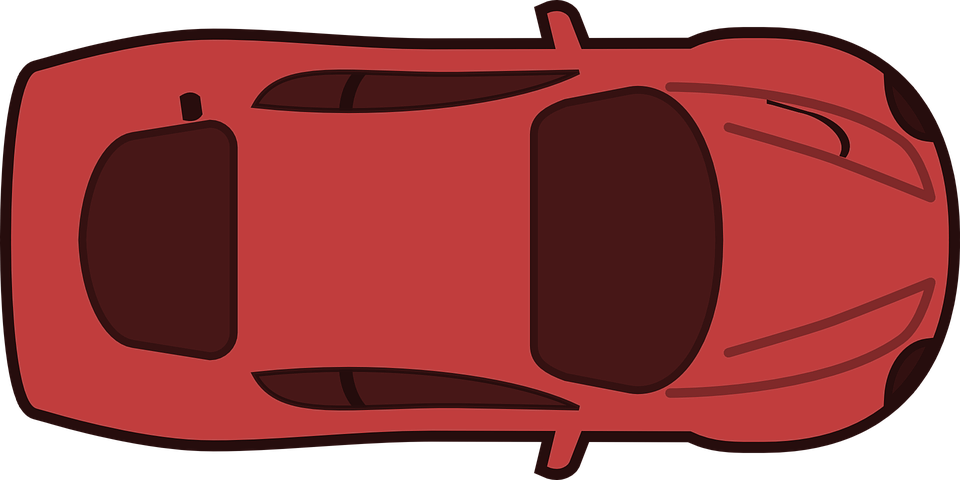
\includegraphics[width=.18\textwidth, angle=0]{figures/ego_car_top_down.png}};
		\draw[->] ([yshift=0.2cm]ego_car.east) -- node[above] {$p_\mathrm{ego}, v_\mathrm{ego}$} ($ (ego_car) + (2.5,0.2)$ );
		% \draw[|-|] ([yshift=-0.2cm]ego_car.east) -- node[below] {$p_{ego}$} (-1,-0.2);
	
		% \node[inner sep=0pt] (target_car_3) at (0,7)
		% {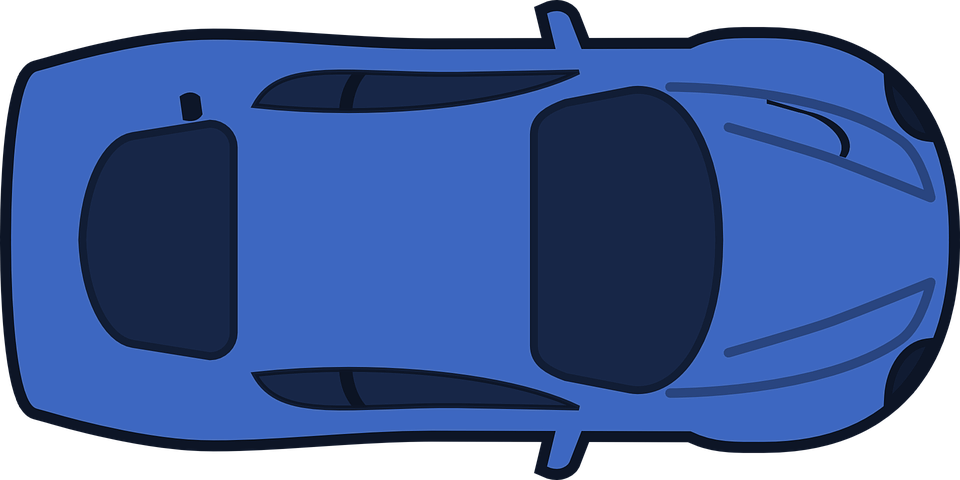
\includegraphics[width=.18\textwidth, angle=-90]{figures/target_car_top_down.png}};
		% \node (tc_text3a) [right=of target_car_3, align=center] {Car $n$};
		% % \node (tc_text3b) [left=of target_car_3, align=center] {Conflict Car};
		% \draw[->] ([xshift=-.3cm]target_car_3.south) -- node[right] {$p_{n} v_{n} \zeta_n$} ($ (target_car_3) + (-.3,-2)$ );
		% \draw[|-|] ([xshift=-0.8cm]target_car_3.south) -- (-.8,1);
		% \node (tc_tti) [below left= 0.9cm and -0.7cm of target_car_3, align=center] {$p_n$  \\ $\tau_{int}$};
	
		\node[inner sep=0pt] (target_car_2) at (0,3.5)
		{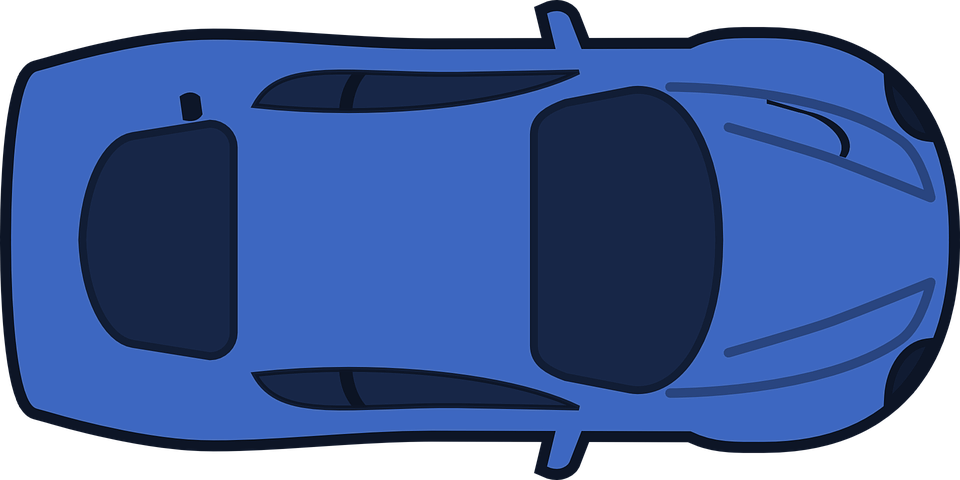
\includegraphics[width=.18\textwidth, angle=-90]{figures/target_car_top_down.png}};
		\node (tc_text2) [right=of target_car_2] {Car $n$};
		\draw[->] ([xshift=-.3cm]target_car_2.south) -- node[right] {$p_{n} v_{n} \zeta_n$} ($ (target_car_2) + (-.3,-2)$ );
		
		\node[inner sep=0pt] (target_car_1) at (0,-1.5)
		{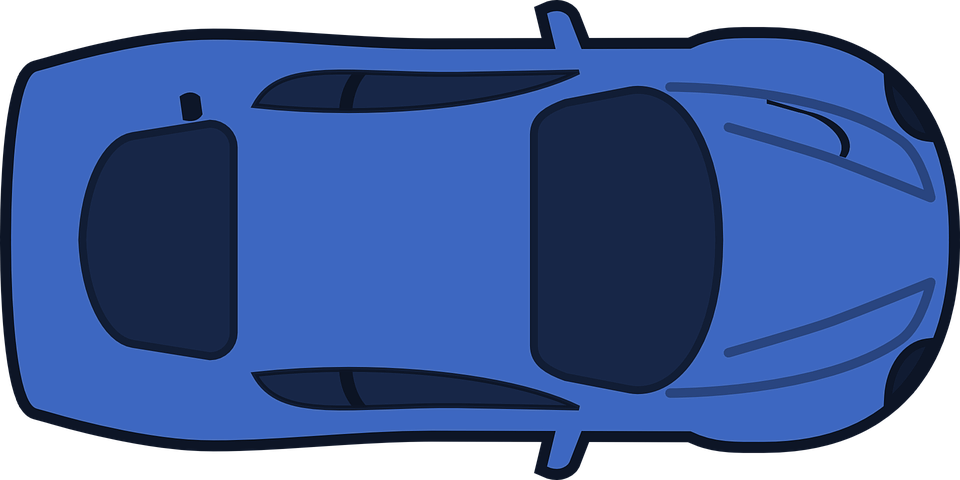
\includegraphics[width=.18\textwidth, angle=-90]{figures/target_car_top_down.png}};
		\node (tc_text1) [right=of target_car_1] {Car 1};
	
	\end{tikzpicture}
	\caption{General description of the states in a simple intersection. The ego vehicle in red is controlled by the agent, while the blue vehicles are the other vehicles crossing the same intersection. Each blue vehicle is described by an index $n$, a position $p_n$, a velocity $v_n$  and hidden intention $\zeta_n$}.
	\label{fig:intersection_scenario}
	\end{figure}

From Section~\ref{sec:background_mdp}, the state space contains all the information necessary about the agent and environment to be able to transition from any given state $s$ to the next state $s'$. In the scenario shown in Figure~\ref{fig:intersection_scenario}, the red car on the horizontal lane represents the ego vehicle controlled by the agent while the blue cars on the vertical lane are the other vehicles which the ego vehicle needs to interact with in order to cross the intersection. 

A simplified description of the state, 
\begin{align}
	s = (p_\mathrm{ego}, v_\mathrm{ego}, \{p_{n}, v_n, \zeta_n\}_{n=1}^N), 
	\label{eq:state}
\end{align}
consists of positions state $p_\mathrm{ego}$ and $p_n$, where subscript \textit{ego} and $n$ denotes the ego vehicle and the index of the surrounding vehicle up to $N$ vehicles. 
% Let's start by defining the information needed. 
Instead of using a Cartesian coordinate system to describe the position $p_\mathrm{ego}$ and $p_n$, relative distance measures are proposed. This way, the state space is generalizable to different intersection designs, e.g., the angle of incidence and the number of crossing points. 
The velocity of ego $v_\mathrm{ego}$ and of all the other traffic participants $v_n$ are also necessary to be able to predict what position they will be in the next state. Finally, the intention of all the other participants $\zeta_n$. As mentioned in Section \ref{sec:intro_intersections}, $\zeta_n$ encapsulates information such as stop sign, traffic light or even inattention in to one variable. 
\paperBelief \ shows a comparison between two fully observable \gls{mdp}s, one with intention and the other one without and the results show that having an intention state reduce number of collisions. 
\paperLSTM \ used a \gls{lstm} network architecture to implicitly predict $\zeta$. %The states describing ego and other vehicle are spearated. Repeat the states for each other vehicle we observe. 

\subsection{Action space}
\label{sec:pomdp_actionspace}
One limitation of deep Q-learning is the requirement for a discrete action space. In various \gls{ad} studies \cite{bouton2019}, it is common practice to define the action space in terms of different acceleration requests. The approach in \paperLSTM \ proposes using short-term goals as actions: \{\textit{`take way', `yield', `follow car~$\{1, \dots , N\}$'}\}.

These short-term goals represent high-level objectives, such as driving through an intersection (take way), stopping at the start of an intersection (yield) or drive behind a specific car (follow car~$n$). Each high-level action is translated into a set of parameters that are input into a sliding mode controller in \paperLSTM \ and a \gls{mpc} in \paperMPC, which then generates the appropriate acceleration to control the ego car.

\subsection{Transition model}
\label{sec:pomdp_transistionmodel}
The transition model is initially unknown, and \gls{rl} is employed to implicitly learn this model by taking actions in the environment from different states, recording the resulting rewards, and noting the subsequent state transitions. In this work, the environment is a simulator, and the primary objective for the agent is to learn the transition dynamics of other vehicles, which depend on their intentions $\zeta$. These intentions are modeled as predetermined actions, governed by an \gls{idm}. Using the \gls{idm} to guide predetermined actions makes the interactions between vehicles more complex, which complicates the learning process. For more details on the simulation environment see Chapter~\ref{ch:simulation_env}.


\subsection{Observation model}
The observation space is closely aligned with the state space $\mathcal{S}$, but it includes some added noise and excludes the intention state $\zeta_n$, because current sensors cannot directly detect the intentions of other drivers.
The observation
\begin{align}
	o = (p_\mathrm{ego}, v_\mathrm{ego}, \{\hat{p}_{n}, \hat{v}_n\}_{n=1}^N), 
	\label{eq:thesis_observation}
\end{align}
encompasses all observable elements of the state, detailed in~\eqref{eq:state}. 
The ego vehicle accurately observes its own states, while it observes noisy measurements of the positions $\hat{p}_{n}$ and velocities $\hat{p}_{n}$ of the surrounding vehicles. These measurements are given by:
\begin{align}
    \label{eq:thesis_noise_pos}
    \hat{p}_{n} = p_{n} + \epsilon_\mathrm{p},\\ 
    \hat{v}_n = v_n + \epsilon_\mathrm{v}
    \label{eq:thsis_noise_vel}
\end{align}
where, $\epsilon_\mathrm{p} \sim \mathcal{N}(0, \sigma^2_p)$ and $\epsilon_\mathrm{v} \sim \mathcal{N}(0, \sigma^2_v)$. 


\subsection{Reward function}
The design of the reward function is pivotal as it determines the value associated with each state, ultimately shaping the driving policy of the agent. A well-crafted reward function is instrumental in guiding the agent towards achieving its objectives effectively.
The reward model in this work is formulated based on terminal states, including reaching the goal, collision events, and timeouts. These terminal states play a critical role in defining the success or failure of the agent's driving behavior and are accordingly reflected in the reward structure.

% \todo{shouldn't you give a concrete example here? Or at least comment on the different designs in the different papers if they are different.}

\section{Simulation environment}
\label{ch:simulation_env}
The simulation environment in this thesis, first introduced in \paperLSTM, places an agent at an intersection tasked with reaching the goal across the intersection while interacting with up to $N$ other cars on the intersecting lane. At the beginning of each episode, up to $N$ vehicles are initialized with initial positions $p_n^0$ distributed along the intersecting lane, starting velocities $v_n^0$ and a deterministic policy that defines their intention $\zeta_n$. 
Each vehicle, including the ego vehicle, adheres to the \gls{idm} (Section~\ref{ch:idm}) aimed at maintaining specific speeds and safe distances, with the maximum acceleration is capped at $5 m/s^2$ to ensure comfort and safety under normal driving conditions.
For example, if a vehicle's intention $\zeta_n$ is yield, it would set the \gls{idm} for the distance to the object in front  $d_n$ to the distance to the start of the intersection, and its velocity $v_{n-1}$ would be set to $0$. Alternatively, a vehicle with a take way intention would follow the IDM only considering the vehicle directly in front of it.

During the simulation, whenever a vehicle in the perpendicular lane crosses the intersection, it is removed from the environment. Subsequently, a new vehicle is spawned at the start of that lane at a random time, with new initial values for position $p_n^0$, velocity $v_n^0$, desired velocity $v^\mathrm{desired}_n$ and intention $\zeta_n$. 
This dynamic spawning process ensures that the traffic scenario continually evolves, presenting varying challenges and interactions for the agent navigating the intersection.
Each episode continues until a terminal state is reached, which can be reaching the goal, collision, safe stop, or deadlock. Rewards are assigned based on a predefined reward function designed to reinforce desired behaviors.


\section{Deep Q-learning approach}
% \todo{In this section, I think you need to give more detail about the methods e.g. detail the DQN structure, explain the MPC in a bit more details. I think this will help understand the section 4.4. }
To find a driving policy $\pi$ for the \gls{pomdp} detailed in the previous section, both \paperLSTM \ and \paperMPC \ used deep Q-learning, described Chapter~\ref{ch:q-learning}. \paperLSTM \ proposed a \gls{dqn} structure with shared weights and \gls{lstm} layer to approximate the Q-function. The shared weight effectively reduces the input space, as the state for each car $n$ can be initially weighted the same as any other car, independent of the order it comes into the neural network. While the \gls{lstm} layer has the role of utilizing the previous states to implicitly estimate a hidden state that could possibly encapsulate the intention of other cars.

As mentioned in Chapter~\ref{sec:pomdp_actionspace}, the actions in \paperLSTM \ are controlled by a sliding mode controller while \paperMPC \ uses an \gls{mpc} to generate a velocity profile for a short time horizon. Instead of specifying which car to drive behind, the action in this context determines which gap between cars the vehicle should drive through. This gap is then translated into constraints that the \gls{mpc} uses to create the velocity profile.

\gls{mpc} excels at creating plans within given constraints but faces challenges with mixed integer problems, making the calculation of the optimal path for all possible actions computationally intensive. On the other hand, Q-learning is effective at estimating the value of an action given a state, but it requires exploring many suboptimal actions before converging on a good one. By combining \gls{rl} and \gls{mpc}, an agent can efficiently select a good action, which the \gls{mpc} can then use to generate a safe and efficient velocity profile.

The agents from \paperLSTM \ and \paperMPC \ are evaluated on both a single intersection, shown in Figure~\ref{fig:example_intersections}\subref{fig:single_intersection}, and a double intersection with two crossing points, shown in Figure~\ref{fig:example_intersections}\subref{fig:double_intersection}. The results are summarized in Table~\ref{tab:results_single_double_crossing}.

\section{Results from simulation}
\label{sec:results_dqn}
% \todo{I am a bit confused here, in the previous sentence you mention 96% success, here 3/4=75%, are you discussing another scenario?}
% \todo{you might want to acknowledge the 4% of cases where it fails and mention some strategies or that it should be addressed in future work.}
The results from Table~\ref{tab:results_single_double_crossing} show that the proposed \gls{dqn} agent from \paperLSTM \ found a policy that successfully crossed a single intersection $96.1\%$ of the time, with $2.8\%$ resulting in collisions and $1.1\%$ resulting in timeouts. 
When comparing agents trained with and without an \gls{lstm} layer, those with the \gls{lstm} succeeded in 3 out of 4 attempts where those without it would fail.
This demonstrates that deep Q-learning has great potential for creating decision-making agents capable of navigating intersections. Additionally, the results from Figure~\ref{fig:results_shared} indicate that using a network structure with shared weights between cars significantly improved the convergence speed of the network. Shared weights, along with other enhancements like dropout and experience replay, are essential components for this improvement.
% \todo{For me, it is obvious what this means, but probably not for your thesis readers. You have not really introduced network structure before. If you want to mention some results here, probably you want to discuss the structure? Or at least refer to the paper where you introduce the structure. Something like. "One of the contribution of this thesis is to propose network architectures that are particularly well suited to the intersection navigation problem. In paper X, we propose an architecture with shared weights to process the information about each observed vehicle. Figure 4.2 ... "}

\begin{figure}[!ht]
	\centering
	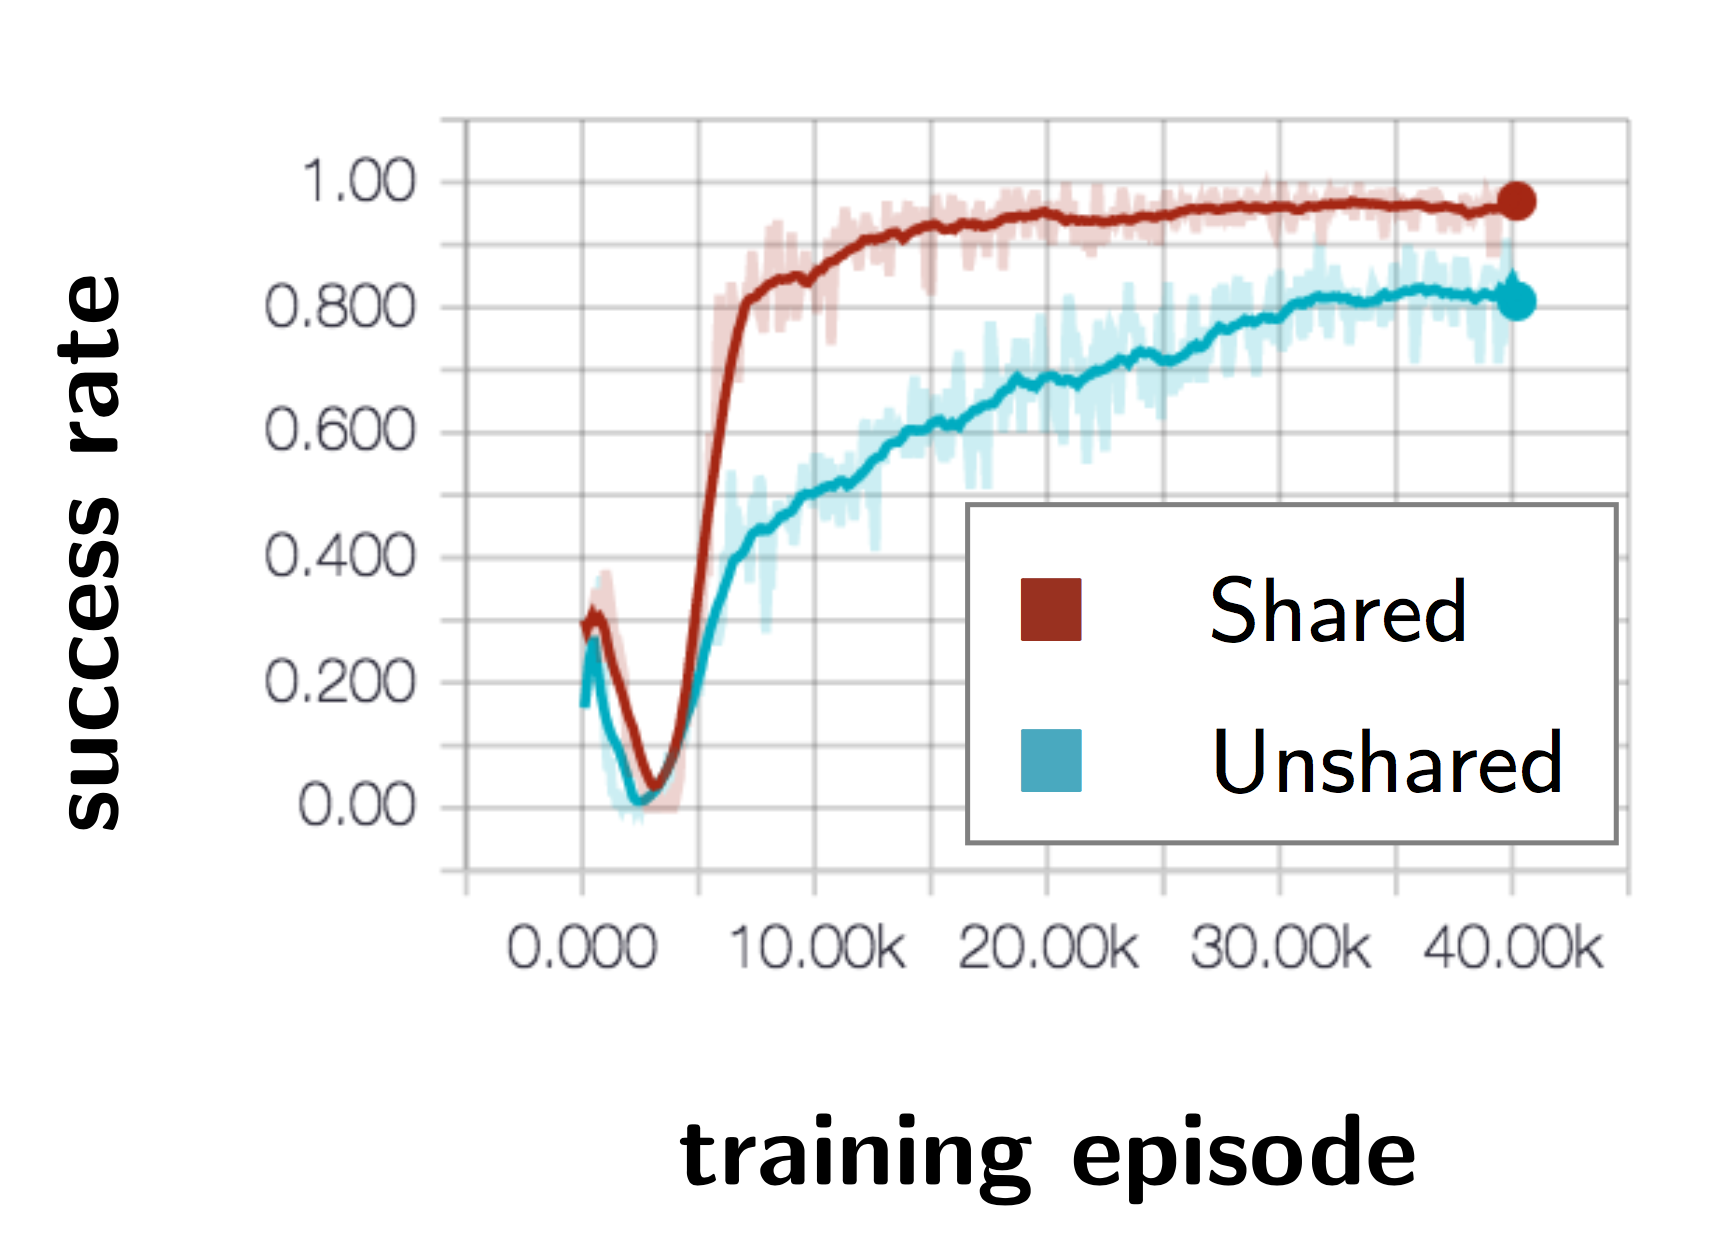
\includegraphics[width=0.7\columnwidth]{YourThesis/papers/lstm/figures/results_shared.png}
	\caption{The figure shows that the success rate for a network with shared weights (brown line) converge faster than the fully connected network structure which do not share weights (turquoise line).}
	\label{fig:results_shared}
\end{figure}

% \todo{This whole paragraph is a bit hard to follow because one needs to have read paper A and paper B. If you want to have this I think you need to add some paragraphs describing on a high level the methods of paper A and paper B.}
As mentioned previously, the controller from \paperLSTM \ could only consider one car at a time, which placed a heavy burden on the \gls{dqn} compensate by frequently switching actions. 
In contrast, in \paperMPC, the \gls{mpc} showed significant improvement in handling more complex intersections.
For instance, in the double intersection, the \gls{mpc} agent succeeded $95.2\%$ of the time with a collision rate of $3.6\%$, compared to the sliding mode controller, which only succeeded $90.9\%$ of the time with a collision rate of $8.3\%$.



% \begin{figure}[!ht]
% 	\centering
% 	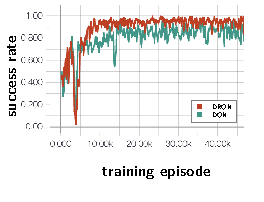
\includegraphics[width=0.7\columnwidth]{figures/figures-recurrent.pdf}
% 	\vspace{-0.5cm}
% 	\caption{Graphs presenting the performance of a DRQN (red) compared to a DQN with a single observation (green), running on scenarios with cars that have different behaviors. When compared a DRQN succeeds in 3 out of 4 attempts, where a DQN fails.}
% 	\label{fig:results_recurremt}
% \end{figure}

% \begin{figure}[t!]
	% \mbox{\parbox{\textwidth}{
% 	\centering
% 	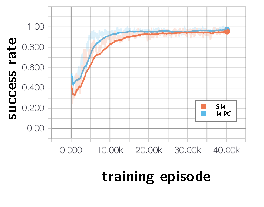
\includegraphics[width=\columnwidth]{YourThesis/papers/mpc/figures/figures-successrate.pdf}
% }}
% 	\caption{Average MPC and SM success rate for a single corssing after evaluating the policy 300 episodes.}
% 	\label{fig:result1}
% \end{figure}

% \begin{figure}[t!]
% 	\centering
% 	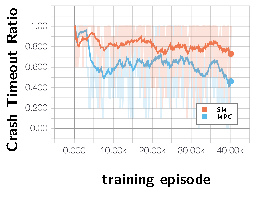
\includegraphics[width=\columnwidth]{YourThesis/papers/mpc/figures/figures-crashratio.pdf}
% 	\vspace{-4em}
% 	\caption{Average MPC and SM crash to timeout ratio for a single crossing after evaluating the policy in 300 episodes. A CTR of $0$ means that all failures are timeouts, while a CTR of $1$ means that all failures are collisions.}
% 	\label{fig:result2}
% \end{figure}

\begin{table}[h]
	\mbox{\parbox{\textwidth}{
	\centering
	\begin{tabular}{ |p{2,6cm}||p{1,2cm}|p{1,2cm}|p{1,2cm}|p{1,2cm}|}
	\hline
	Controller &\multicolumn{2}{|c|}{Success Rate}&\multicolumn{2}{|c|}{Collision Rate}\\
	\hline
	 & Single & Double & Single & Double\\
	\hline
	SM (\paperLSTM) & $96.1\%$ & $90.9\%$ & $2.8\%$ & $8.3\%$\\
	MPC (\paperMPC) & $97.3\%$ & $95.2\%$ & $1.2\%$ & $3.6\%$\\
	\hline
	\end{tabular}
	}}
	\caption{Average success rates and collision rates for a fully trained \gls{dqn} agent driving through a single and double intersections. If the agent failed to reach the goal or collide within a given time, the terminal state was classified as a timeout.}% across single and double crossings.}   
\label{tab:results_single_double_crossing}
\end{table}


\section{Discussion}
% \section{The intersection problem}
\begin{figure}
	\mbox{\parbox{\textwidth}{
		\centering
		\begin{tikzpicture}
			\def\xstart{-7};

			\coordinate (p) at (3,0);
			\foreach \n/\w/\c in {z0/2/green,z1/2/red,z2/2.5/orange,z3/3.5/blue}{
				\node[rectangle,
				draw=none,
				anchor=east,
				text = black,
				fill = \c!60,
				minimum width = \w cm, 
				minimum height = 2cm] 
				(n) at (p) {\Huge \n};
				
				\coordinate (p) at (n.west);
			}

			% Crossing
			\draw[line width=0.5mm] (\xstart, 1) -- (-1, 1) -- (-1, 5);
			\draw[line width=0.5mm] (\xstart, -1) -- (-1, -1) -- (-1, -2);
			\draw[line width=0.5mm] (1, 5) -- (1, 1) -- (3, 1);
			\draw[line width=0.5mm] (1, -2) -- (1, -1) -- (3, -1);
			
			% cars
			\node[inner sep=0pt] (ego_car) at (-7,0)
			{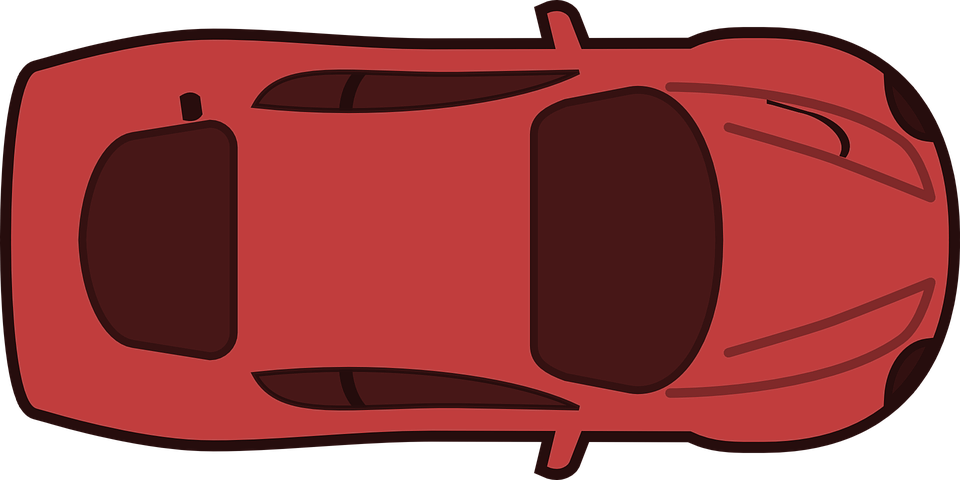
\includegraphics[width=.18\textwidth, angle=0]{figures/ego_car_top_down.png}};
			\node[inner sep=0pt] (target_car) at (0,4)
			{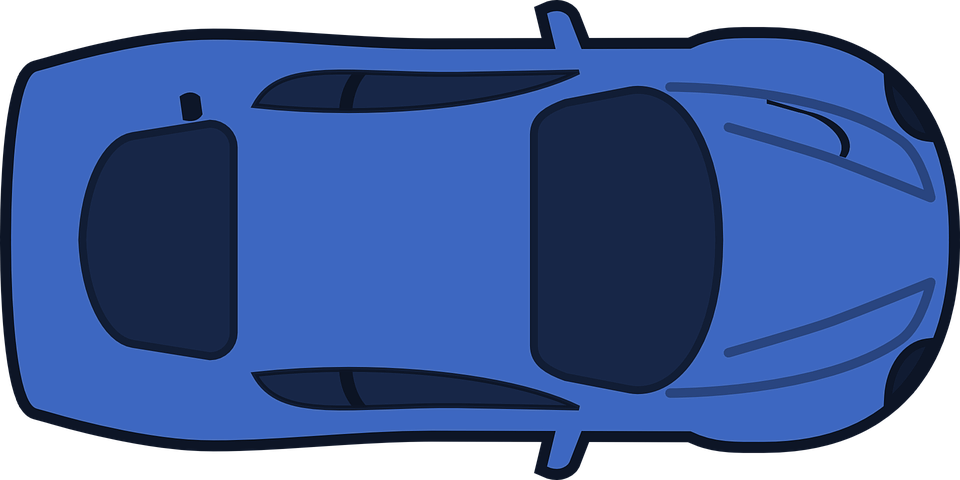
\includegraphics[width=.18\textwidth, angle=-90]{figures/target_car_top_down.png}};

	\end{tikzpicture}
	}}
	\caption{Intersection scenario divided into zones describing what is required of the decision maker in different zones}
	\label{fig:zones}
\end{figure}

Observing the behavior of a fully trained agent from \paperLSTM \ and \paperMPC \ provides the insight that the path of the ego vehicle can be segmented into four zones, illustrated in Figure~\ref{fig:zones}. Starting from the right, Zone 0 represents the \textit{safe zone}, where the ego vehicle is out of danger and can resume nominal driving. Zone 1 is the \textit{conflict zone}, where a collision with another vehicle is possible. Zone 2, the \textit{critical decision zone}, is the final opportunity for the vehicle to either stop or proceed through the intersection. The size of zone 2 is determined by the minimum distance required for the vehicle to come to a complete stop before entering the conflict zone, ensuring sufficient time for safe decision-making. Lastly, Zone 3, the \textit{information gathering zone}, is situated furthest from the intersection. Here, the agent can observe how other vehicles behave over time to estimate their intentions.

The goal is to reach Zone 0. To achieve this, the agent aims to minimize the time spent in Zone 1 if there is a chance of intersection with another car. Our actions are formulated as short-term goals, designed for comfortable use with lower acceleration rates. The size of Zone 2 depends on the vehicle's current speed, which is influenced by its behavior in Zone 3.

Now, two conflicting strategies emerge: to minimize time in Zone 1, the agent desires a high speed entering the intersection. However, it also seeks a low speed to reduce the size of Zone 2 and the critical decision period. If the intentions of other vehicles are known, the stochasticity in Zone 1 would be eliminated, transforming the problem into a scheduling task aimed at creating a velocity profile that minimizes the time required to cross. However, since the intentions of other vehicles are inherently stochastic, the next chapter offers a promising approach by accounting for this uncertainty and optimizing decision-making in dynamic traffic scenarios.



\chapter{Learning without a model}
\begin{center}
\textit{\textbf{RQ 1: How can RL be used to create a decision-making agent for autonomous driving through an unsignalized intersection?}}
\end{center}
\vspace{12pt}
\tommy{Deep Q-learning approach}
We want to formulate the problem in such a way that abstracts the information of traffic lights, traffic signs and intention. This way the car is closer to L5 by not relying on the different traffic lights.

One motivation example is in how traffic lights works. In Sweden, we have sensors that can sense if there are cars in an intersection and create a traffic light schedule accordingly, compared to the US where the traffic signals set up using timers. As a consequence, Drivers approaching a yellow light 

The \gls{dqn} algorithm uses a \gls{nn} and has two disadvantages. One is that the size of the network is fixed, this forces the input space to be fixed. Our state space is defined by the physical state of the surrounding cars, and the number of cars we observe at each situation variate. %Therefor we need a way to invariate of 

\section{Approach (State representation, observable and unobservable)}
This paper explored the possibility of solving the problem with \gls{rl} by trying a verity of different methods from the rainbow paper with the addition to the LSTM layer and presented the results that had the highest impact on the conversion. 
\todo{State representation}
This section describes the general state representation used in this research that enables these methods to be generalizable for different type of intersection and crossings. 
By describing the state space as a set of distances to intersection points, we can abstract the map layout of different intersections and the same algorithms would work for intersections variations that we haven't specifically trained on. 
\todo{add image of intersection scenario with 90 degree entry point and 45 degree entry point.}
\todo{Observable states}
Position, velocity and acceleration. 
\todo{Unobservable states}
Intentions. Traffic lights and traffic signs. 
\todo{explain rewards}
large negative reward for invalid actions.
\section{Simulated experiments}
\section{Results and discussion}
\begin{itemize}
  \item STG as actions
  \item shared weights
  \item effect of replay, dropout 
  \item comparing a dqn and Drqn 
\end{itemize}
however sensitive to noise. 

LSTM take into account the history, but when applied in the real world with noise the model did not perform as well. 
The immidiate reward for jerk is 
\tommy{finding time to intersection and position itself in a way that does not conflict with other cars.}

\tommy{FIND A SECTION. Collisions in this thesis, may sound critical and extreme. But collisions in this content is for the purpose of the simulator and for the terminal state of the agent. Translated to a system perspective, it would mean that a backup collision avoidance algorithm had to interfere and in the worst case take over. }

% !TEX root=../../Thesis.tex
\newcommand {\matr}[2]{\left[\begin{array}{#1}#2\end{array}\right]}
\newcommand{\E}{\mathbb{E}}
\newcommand{\tr}{\mathrm{tr}}
\newcommand{\x}{{\mathbf{x}}}
\renewcommand{\u}{{\mathbf{u}}}
\newcommand{\w}{{\mathbf{w}}}
\renewcommand{\r}{{\mathbf{r}}}


\chapter{Combining reinforcement learning and model based optimization}\label{ch:mpc}
\begin{center}
\textit{\textbf{RQ 3: How do can a \gls{rl} agent handle situations it has not been trained on?}}
\end{center}
\vspace{12pt}

\todo{as we see in previous chapter }

\section{MPC}
\todo{rewrite}
\gls{mpc} is an optimization-based control technique where an Optimal Control Problem~(OCP) is repeatedly solved over a receding limited time horizon, starting from the current system state. In particular, for every time instance, a mathematical model of the controlled system is used to simulate the future states over a finite horizon, while a sequence of control inputs are selected and optimized given an objective cost function. The first element in the sequence of control inputs is then applied to the real system, and a new OCP with an updated state is solved at the next time instance.

\section{Approach, (Action space, options. MPC)}
\tommy{Mixed-Integer Programming (MIP) Problems
A mixed-integer programming (MIP) problem is one where some of the decision variables are constrained to be integer values (i.e. whole numbers such as -1, 0, 1, 2, etc.) at the optimal solution.  
However, integer variables make an optimization problem non-convex, and therefore far more difficult to solve.  Memory and solution time may rise exponentially as you add more integer variables.}

MPC has a mixed integer problem, calculating the optimal path for all possible action is very computationally heavy. 
RL DQN. Only has discrete actions. Can not guarantee safety but is good at choosing actions with the best utility (value). 
The reward function takes in the predicted outcome of the model in the MPC and can penalize the choice of action. but if experience show that the outcome is better than the model, it can choose to take a bad action that would lead to a better total reward compared to only following a conservative model. 

\tommy{in this work we simulate three different intention agents, take way, give way and cautious agent.}
\begin{figure}[t!]
	\mbox{\parbox{\textwidth}{
	\centering
	% \vspace{0.3cm}
	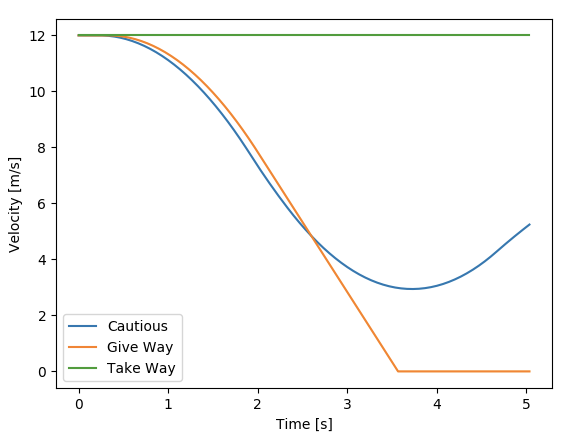
\includegraphics[width=0.7\columnwidth]{YourThesis/papers/mpc/figures/velocity_profiles_agents.png}
	}}
	\caption{Example of how velocity profile of the different intention agents can look like. All agents have the same starting velocity of $12$m/s and are approaching the same intersection}
	% \label{fig:intention_profiles}
	% \vspace{-0.3cm}
\end{figure}\
\todo{reward function}
added Q masking.
Q-masking reduce the search space, in this work we showed it for unavailable actions but could be extended to actions limited by the precautionary safety module. 
By combining the having the \gls{mpc} cost as a negative reward the \gls{dqn} can balance the control cost with the high level goal of reaching the goal and even choose an action that is on average good on a high level but may not seem that way to the \gls{mpc}.

Given the state representation, the dynamics of the vehicle is then modeled using a  triple integrator with jerk as control input.

\tommy{mpc cost function}
The objective of the agent is to safely track a reference, e.g. follow a path with a target speed, acceleration, and jerk profile, while driving comfortably and satisfying constraints that arise from physical limitations and other road users, e.g. not colliding in intersections with crossing vehicles. Hence, we formulate  the  problem as a finite horizon, constrained optimal control problem
\begin{subequations}
	\label{eq:mpc2}
	\begin{align}
	J = \min_{\bar\x,\bar\u} & \sum_{k=0}^{N-1}% \varphi_n(x_n,u_n) + \varphi_N(x_N)\\
	\matr{c}{\bar\x_k - \r_k^\x \\ \bar\u_k - \r_k^\u}^\top \matr{cc}{Q &S^\top\\S & R} \matr{c}{\bar\x_k - \r_k^\x \\ \bar\u_k - \r_k^\u} \\
	&\qquad + \matr{c}{\bar\x_N - \r_N^\x}^\top P \matr{c}{\bar\x_N - \r_N^\x}\nonumber\\
	&\text{s.t.}\ \ \, \bar\x_0 = \hat{\x}_0, \label{eq:mpcState2}\\
	&\qquad{}\bar\x_{k+1} = A\bar\x_{k}+B\bar\u_{k},\label{eq:mpcDynamics2}\\
	&\qquad{}h(\bar\x_k,\bar\u_k,\bar{\mathbf{o}}_k,a_k) \leq{} 0, \label{eq:mpcInequality2}
	\end{align}
\end{subequations}
where $k$ is  the prediction time index, $N$ is the prediction horizon, $Q$, $R$, and $S$ are the stage costs, $P$ is the terminal cost, $\bar\x_k$ and $ \bar\u_k$ are the predicted state and control inputs, $\r^\x_k$ and $\r^\u_k$ are the state and control input references, $\bar{\mathbf{o}}_k$ denotes the predicted state of vehicles in the environment which need to be avoided, and $a$ is the action from the high-level decision maker. Constraint \eqref{eq:mpcState} enforces that the prediction starts  at the current state estimate $\hat\x_0$, \eqref{eq:mpcDynamics} enforces the system dynamics, and \eqref{eq:mpcInequality} enforces constraints on the states, control inputs, and obstacle avoidance.

The reference points, $\r^\x_k$, $\r^\u_k$ are assumed to be set-points of a constant velocity trajectory, e.g. following the legal speed-limit on the road. Therefore, we set the velocity reference according to the driving limit, and the acceleration and jerk to zero.


% \tommy{Obstacle prediction}
% In order for the vehicle planner in \eqref{eq:mpc} to be able to properly avoid collisions, it is necessary to provide information about the surrounding vehicles in the environment. Therefore, similarly to \cite{batkovic2019}, we assume that a sensor system provides information about the environment, and that there exists a prediction layer which generates future motions of other vehicles in the environment. The accuracy of the prediction layer will heavily affect the performance of the planner, hence, it is necessary to have computationally inexpensive and accurate prediction methods.

% In this paper, for simplicity the future motion of other agents is estimated by a constant velocity prediction model. The motion is predicted at every time instant for prediction times $k\in[0,N]$, and is used to form the collision avoidance constraints, which we describe in the next section. Even though more accurate prediction methods do exist, e.g. \cite{lefevre2014survey,batkovic2018}, we use this simple model to show the potential of the overall framework.

% \tommy{Collision avoidance}
% % \begin{figure}[t]
% % 	\centering
% % 	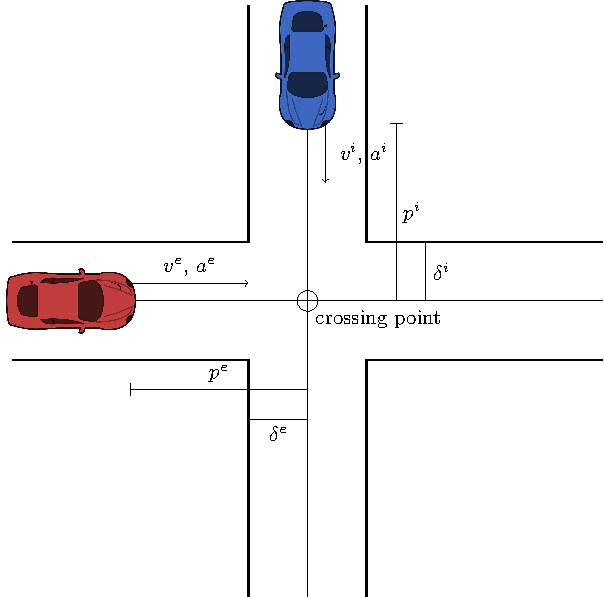
\includegraphics[width=0.6\columnwidth]{figures/figures-observations.pdf}
% % 	\caption{Observations of a scenario}
% % 	\label{fig:observations2}
% % \end{figure}\
% We denote a vehicle $j$ with the following notation $\x^j:=[p^j\, v^j\, a^j]^\top$, and an associated crossing point at position $p^{\mathrm{cross},j}$ in its own vehicle frame, which translated into the ego-vehicle frame is denoted as $p^{\mathrm{cross},j}_\mathrm{ego}$. With a predefined road topology, we assume that the vehicles will travel along the assigned paths, and that collisions may only occur at the crossing points $p^{\mathrm{cross},j}$ between an obstacle and the ego vehicle. Hence, for collision avoidance, we use the predictions of the future obstacle states $\bar\x^j_k$ for times $k\in[0,N]$, provided by a prediction layer outside of the MPC framework. Given the obstacle measurements, the prediction layer will generate future states throughout the prediction horizon. With this information, it is possible to identify the time slots when an obstacle will enter the intersection.

% Whenever an obstacle $j$ is predicted to be within a threshold of $p^{\mathrm{cross},j}$, e.g. the width of the intersecting area, the ego vehicle faces a constraint of the following form
% \begin{gather*}
% \bar{p}_k^\mathrm{e} \geq{} p^{\mathrm{cross},j}_\mathrm{ego} + \Delta,\quad\underline{p}_k^\mathrm{e} \leq{} p^{\mathrm{cross},j}_\mathrm{ego} - \Delta,
% \end{gather*}
% where $\Delta$ ensures sufficient padding from the crossing point that does not cause a collision. The choice of $\Delta$ must be at least such that $p_k$ together with the dimensions of the ego-vehicle does not overlap with the intersecting area.

% \tommy{Take way and give way constraint}
% Since the constraints from the surrounding obstacles become non-convex, we rely on the high-level policy maker to decide through action $a$ how to construct the constraint \eqref{eq:mpcInequality} for Problem \eqref{eq:mpc}. The take-way action implies that the ego-vehicle drives first through the intersection, i.e., it needs to pass the intersection before all other obstacles. This implies that for any vehicle $j$ that reaches the intersection during prediction times $k\in[0,N]$, the generated constraint needs to lower bound the state $p_k$ according to
% \begin{equation}
% \max_{j}p^{\mathrm{cross},j}+\Delta \leq{}p_k^\mathrm{e}.
% \end{equation}
% Similarly, if the action is to give way, then the position needs to be upper bounded by the closest intersection point so that
% \begin{equation}
% p_k^\mathrm{e} \leq{} \min_{j}p^{\mathrm{cross},j}_\mathrm{ego}-\Delta,
% \end{equation} 
% for all times $k$ that the obstacle is predicted to be in the intersection.

% \tommy{Following an obstacle}
% For any action $a$ that results in the following of an obstacle $j$, the ego-vehicle position is upper bounded by $p^\mathrm{e}_k \leq{} p^\mathrm{cross,j}_\mathrm{ego}$. We construct constraints for obstacles $i\neq{}j$ according to
% \begin{itemize}
% 	\item if $p^\mathrm{cross,i}<{}p^\mathrm{cross,j}$ then $p^\mathrm{cross,i}+\Delta\leq{}p_k^\mathrm{e}$, which implies that the ego-vehicle should drive ahead of all obstacles $i$ that are approaching the intersection;
% 	\item if $p^\mathrm{cross,i}>{}p^\mathrm{cross,j}$ then $p_k^\mathrm{e}\leq{}p^\mathrm{cross,i}-\Delta$, which implies that the ego-vehicle should wait to pass obstacle $j$ and other obstacles $i$;
% 	\item if $p^{\mathrm{cross,i}}=p^{\mathrm{cross},j}$ then the constraints generated for obstacle $i$ becomes an upper or lower  bound depending on if obstacle $i$ is ahead or behind the obstacle $j$ into the intersection.
% \end{itemize}


\section{Simulated experiments}
We show the difference in a multi crossing scenario where the MPC can plan a path for both intersections while our previous DQN only handles one at a time. 

\begin{figure}[t]
	\mbox{\parbox{\textwidth}{
	\centering
	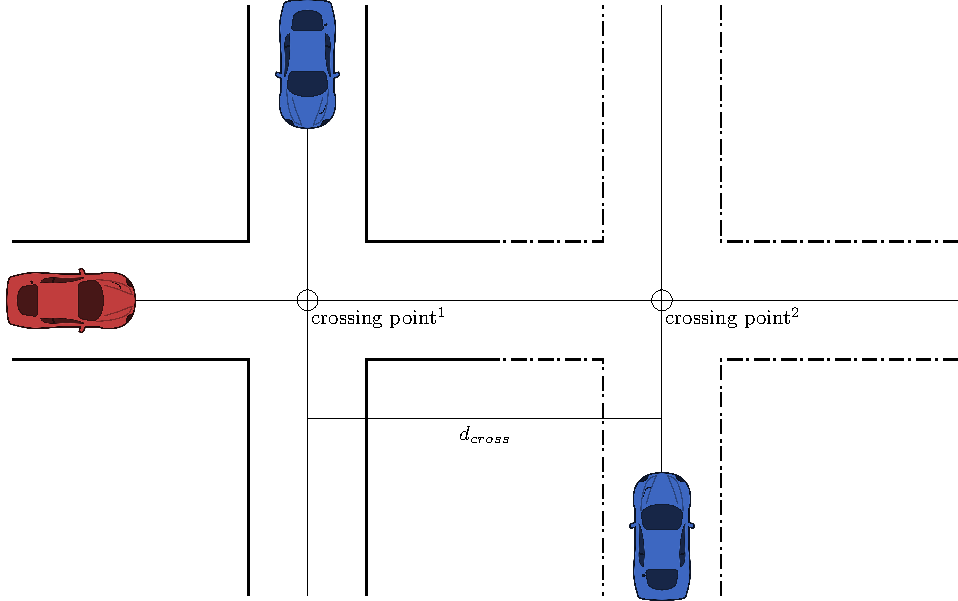
\includegraphics[width=.95\columnwidth]{YourThesis/papers/mpc/figures/figures-scenarios.pdf}
	}}
	\caption{Illustration of a intersection scenario, where the solid line is a single crossing and together with the dashed line creates a double crossing.}
	% \label{fig:scenario}
\end{figure}

\section{Results and discussion}

% \begin{figure}[t!]
	% \mbox{\parbox{\textwidth}{
% 	\centering
% 	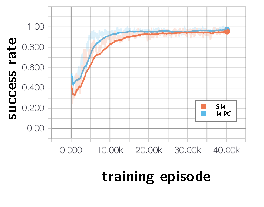
\includegraphics[width=\columnwidth]{YourThesis/papers/mpc/figures/figures-successrate.pdf}
% }}
% 	\caption{Average MPC and SM success rate for a single corssing after evaluating the policy 300 episodes.}
% 	\label{fig:result1}
% \end{figure}

% \begin{figure}[t!]
% 	\centering
% 	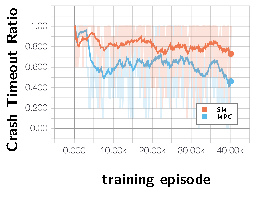
\includegraphics[width=\columnwidth]{YourThesis/papers/mpc/figures/figures-crashratio.pdf}
% 	\vspace{-4em}
% 	\caption{Average MPC and SM crash to timeout ratio for a single crossing after evaluating the policy in 300 episodes. A CTR of $0$ means that all failures are timeouts, while a CTR of $1$ means that all failures are collisions.}
% 	\label{fig:result2}
% \end{figure}

\begin{table}[t!]
	\mbox{\parbox{\textwidth}{
	\centering
	\begin{tabular}{ |p{1,6cm}||p{1,2cm}|p{1,2cm}|p{1,2cm}|p{1,2cm}|}
	\hline
	Controller &\multicolumn{2}{|c|}{Success Rate}
	&\multicolumn{2}{|c|}{Timeout Ratio}\\
	\hline
	 & Single & Double & Single & Double\\
	\hline
	SM & $96.1\%$ & $90.9\%$ & $72\%$ & $93\%$\\
	MPC & $97.3\%$ & $95.2\%$ & $45\%$ & $76\%$\\
	\hline
	\end{tabular}
	}}
	\caption{Average success rates and collision to timeout rates.}% across single and double crossings.}   

% \label{tab:successrate}
\end{table}

synergies between mpc and dqn
% !TEX root=../../Thesis.tex
\chapter{Accounting for the uncertainty}\label{ch:uncertainty}
\todo{Rewrite chapter name}
\begin{center}
	\textit{\textbf{RQ 4: How can the quality of a RL agent be improved by accounting for uncertainty?}}
	\end{center}
	\vspace{12pt}

The motivation of handling uncertainty. In this chapter we present two approches to handling the uncertainty, one is the uncertainty in output of the \gls{dqn} and the other in the uncertainty of the intention estimation that is feed as an input to the \gls{dqn}.


\section{Uncertainty of the decision}
\tommy{NN is a black box. The utility value q that come from the DQN works great if it was trained on the }


\subsection{Approach}
One limitation of the DQN algorithm is that only the maximum likelihood estimate of the $Q$-values is returned. The risk of taking a particular action can be approximated as the variance in the estimated $Q$-value~\cite{Garcia2015}. One approach to obtain a variance estimation is through statistical bootstrapping~\cite{Efron1982}, which has been applied to the DQN algorithm~\cite{Osband2016}. The basic idea is to train an ensemble of neural network on different subsets of the available replay memory. The ensemble will then provide a distribution of $Q$-values, which can be used to estimate the variance. Osband et al. extended the ensemble method by adding a randomized prior function (RPF) to each ensemble member, which gives a better Bayesian posterior~\cite{Osband2018}. The $Q$-values of each ensemble member $k$ is then calculated as the sum of two neural networks, $f$ and $p$, with equal architecture, i.e.,
%
\begin{align}
	Q_k(s,a) = f(s,a;\theta_k) + \beta p(s,a;\hat{\theta}_k).
\end{align}
%
Here, the weights $\theta_k$ of network $f$ are trainable, and the weights $\hat{\theta}_k$ of the prior network $p$ are fixed to the randomly initialized values. A parameter $\beta$ scales the importance of the networks. With the two networks, the loss function in Eq.~\ref{eq:loss} becomes
%
\begin{align}
	\label{eq:loss_boot}
	L(\theta_k) = \mathbb{E}_M \Big[ & (r + \gamma \max_{a'} (f_{\theta^-_k}+\beta p_{\hat{\theta}_k})(s',a') \nonumber \\
	& - (f_{\theta_k}+ \beta p_{\hat{\theta}_k})(s,a) )^2 \Big].
\end{align} 

Algorithm~\ref{alg:training} outlines the complete ensemble RPF method, which was used in this work. An ensemble of $K$ trainable and prior neural networks are first initialized randomly. Each ensemble member is also assigned a separate experience replay memory buffer $m_k$ (although in a practical implementation, the replay memory can be designed in such a way that it uses negligible more memory than a shared buffer). For each new training episode, a uniformly sampled ensemble member, $\nu \sim \mathcal{U}\{1,K\}$, is used to greedily select the action with the highest $Q$-value. This procedure handles the exploration vs. exploitation trade-off and corresponds to a form of approximate Thompson sampling. Each new experience $e = (s_i, a_i, r_i, s_{i+1})$ is then added to the separate replay buffers $m_k$ with probability $p_\mathrm{add}$. Finally, the trainable weights of each ensemble member are updated by uniformly sample a mini-batch $M$ of experiences and using stochastic gradient descent (SGD) to backpropagate the loss of Eq.~\ref{eq:loss_boot}.

\begin{algorithm}[!t]
	\caption{Ensemble RPF training process}\label{alg:training}
	\begin{algorithmic}[1]
		\For{$k \gets 1$ to $K$}
			\State Initialize $\theta_k$ and $\hat{\theta}_k$ randomly
			\State $m_k \gets \{\}$
		\EndFor
		\State $i \gets 0$
		\While{networks not converged}
			\State $s_i \gets $ initial random state
			\State $\nu \sim \mathcal{U}\{1,K\}$%, where $k \in \mathbb{N}$
			\While{episode not finished}
				\State $a_i \gets \argmax_{a} Q_\nu(s_i,a)$
				\State $s_{i+1}, r_i \gets $ \Call{StepEnvironment}{$s_i, a_i$}
				% \For{$i \in \{1,\dotsc,K\}$}
				\For{$k \gets 1$ to $K$}
					\If{$p \sim \mathcal{U}(0,1) < p_\mathrm{add}$}%, where $p \in \mathbb{R}$ 
						\State $m_k \gets m_k \cup \{(s_i, a_i, r_i, s_{i+1})\}$
					\EndIf
					\State $M \gets $ sample mini-batch from $m_k$
					\State update $\theta_k$ with SGD and loss $L(\theta_k)$
				\EndFor
				\State $i \gets i + 1$
			\EndWhile
		\EndWhile
	\end{algorithmic}
\end{algorithm}

\begin{align*}
r_t = &\begin{cases}
1 & \text{at reaching the goal, }\\
-1 & \text{at a collision},\\
-\left(\frac{j_t}{j_{\max}}\right)^2\frac{\Delta \tau}{\tau_\mathrm{max}} & \text{at non-terminating steps.}
% \label{eq:reward}
\end{cases} 
\end{align*}


\tommy{Confidence criterion}

The agent's uncertainty in choosing different actions can be defined as the coefficient of variation\footnote{Ratio of the standard deviation to the mean.} $c_\mathrm{v}(s,a)$ of the $Q$-values of the ensemble members.  
In previous work, we introduced a confidence criterion that disqualifies actions with $c_\mathrm{v}(s,a) > c_\mathrm{v}^\mathrm{safe}$, where $c_\mathrm{safe}$ is a hard threshold~\cite{Hoel2020}. 
The value of the threshold should be set so that $(s,a)$ combinations that are contained in the training distribution are accepted, and those which are not will be rejected. This value can be determined by observing values of $c_\mathrm{v}$ in testing episodes within the training distribution, see Sect.~\ref{sec:resultsWithinDistribution} for further details. 


% A high uncertainty, where $c_\mathrm{v}(s,a) > c_\mathrm{v}^\mathrm{safe}$, indicates that $(s,a)$ is outside the training distribution. The parameter value $c_\mathrm{safe}$ can be set just above the observed values of $c_\mathrm{v}$ in testing episodes within the training distribution, see Sect.~\ref{sec:resultsWithinDistribution} for further details.

When the agent is fully trained (i.e., not during the training phase), the policy chooses actions by maximizing the mean of the $Q$-values of the ensemble members, with the restriction $c_\mathrm{v}(s,a) < c_\mathrm{v}^\mathrm{safe}$, i.e.,
%
\begin{equation}
	\begin{aligned}
		\argmax_{a} \frac{1}{K} \sum_{k=1}^K Q_k(s,a),\\
		\textrm{s.t.} \quad c_\mathrm{v}(s,a) < c_\mathrm{v}^\mathrm{safe}.
	\end{aligned}
\end{equation}
%
In a situation where no possible action fulfills the confidence criterion, a fallback action $a_\mathrm{safe}$ is chosen.



\subsection{Simulated experiments}
\todo{show the difference of having the uncertainty estimate not having the estimate}

\subsection{Results and discussion}
We show two approaches of handing uncertainty. with an estimate of the uncertainty in actions we showed that it can be used to reduce collisions and risk by choosing another policy than the one trained on data it is not confident in. 


\section{Uncertainty of the intention}
In paper A the policy put itself in a position that would not be in conflict with another cars time to intersection and could avoid a lot of the collisions. But the cases the cars collided was when in somehow ended up in a collision course and thats when it had trouble making its way out. 

\subsection{Approach}


Because the state is no longer observable, the agent must reason about the history of taken actions and observations. Often, this history can be summarized in a statistic refered to as a belief, or belief state. A belief is a probability distribution over states so that $b: \mathcal{S} \rightarrow [0,1]$ and $\sum_{s} b(s)=1$, or $\int_{s} b(s)=1$ for continuous states. 

\subsection{Simulated experiments}

\subsection{Results and discussion}

\begin{figure}[!t]
	\mbox{\parbox{\textwidth}{
	\centering
	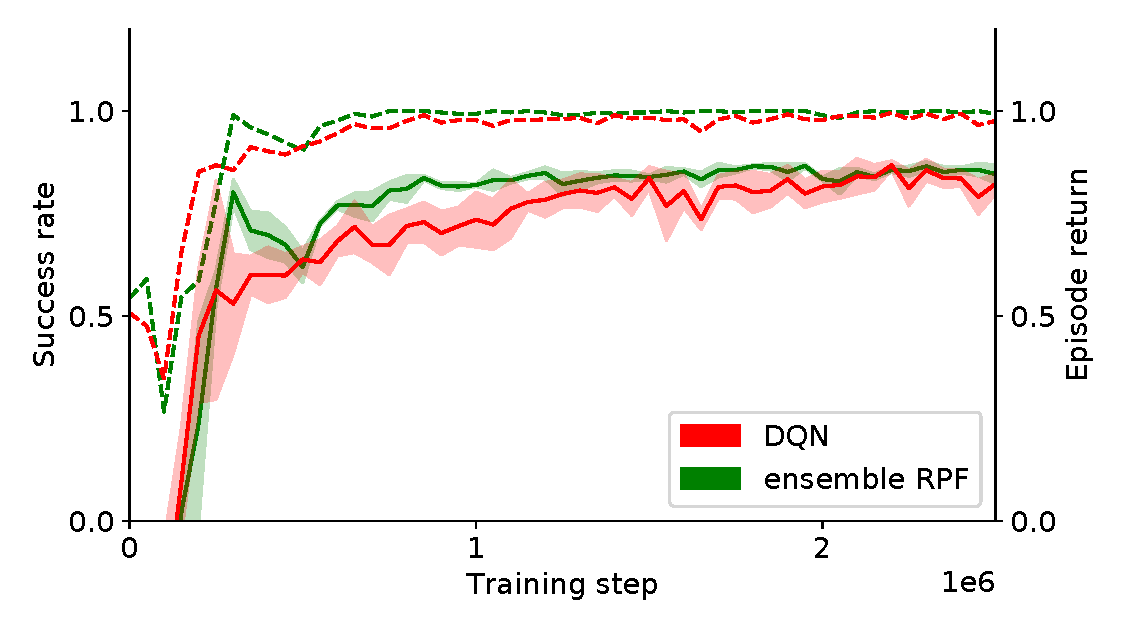
\includegraphics[width=0.99\columnwidth]{YourThesis/papers/ensamble/figures/return_success_rate_2_wo_type_3_fonts.pdf}
	}}
	\caption{Proportion of test episodes where the ego vehicle reached its goal (dashed), and episode return (solid), over training steps for the ensemble RPF and DQN methods. The shaded areas show the standard deviation for $5$ random seeds.}
	% \label{fig:returnAndSuccess}
\end{figure}

% ZZZ Change left y-axis to percent, to make it more clear that it refers to a proportion

\begin{figure}[!t]
	\mbox{\parbox{\textwidth}{
	\centering
		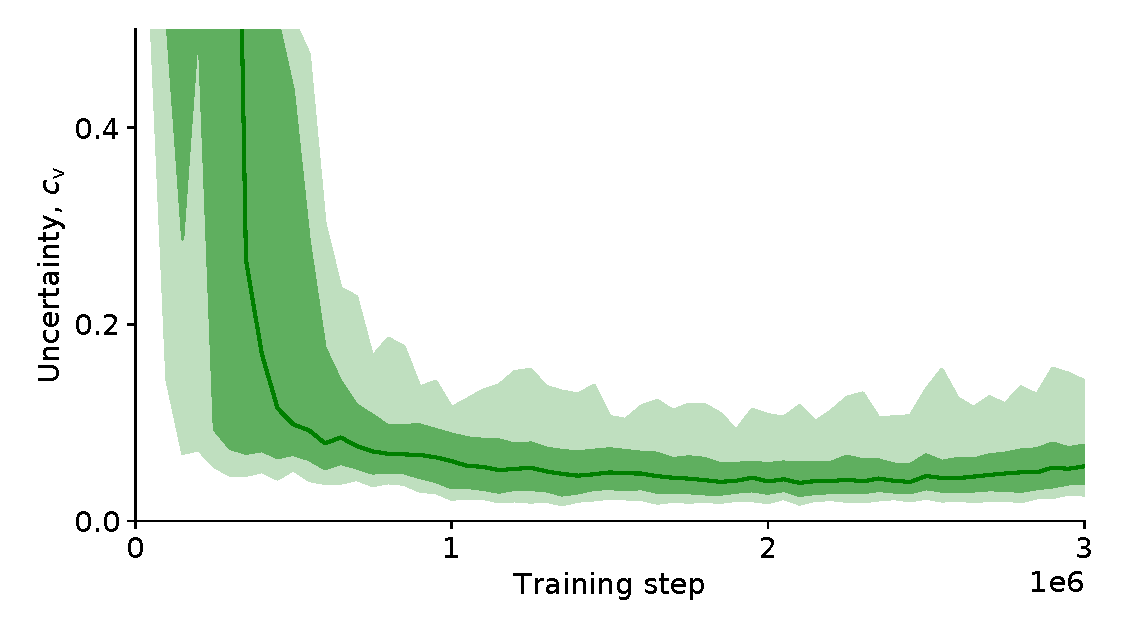
\includegraphics[width=0.99\columnwidth]{YourThesis/papers/ensamble/figures/uncertainty_3_wo_type_3_fonts.pdf}
		}}
		\caption{Mean coefficient of variation $c_\mathrm{v}$ for the chosen action during the test episodes. The dark shaded area shows percentiles $10$ to $90$, and the bright shaded area shows percentiles $1$ to $99$.}
	% \label{fig:cv}
\end{figure}

\begin{figure}[!t]
	\mbox{\parbox{\textwidth}{
	\centering
		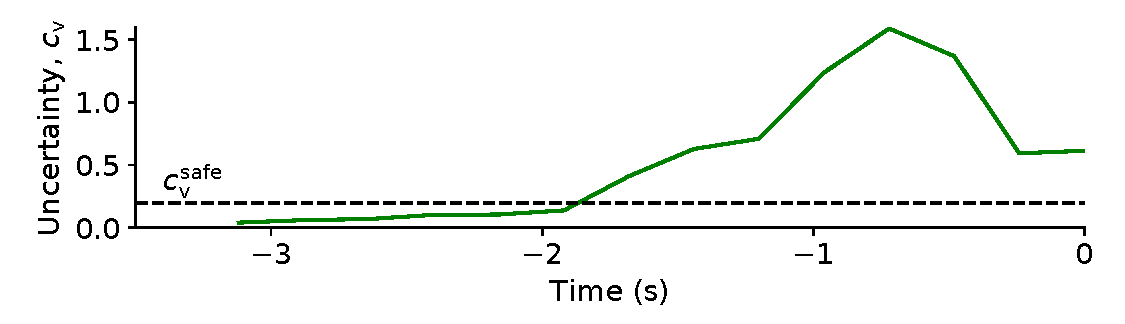
\includegraphics[width=0.99\columnwidth]{YourThesis/papers/ensamble/figures/uncertainty_at_collision_wo_type_3_fonts.pdf}
		}}
		\caption{Uncertainty $c_\mathrm{v}$ during the time steps before one of the collisions in the test episodes, within the training distribution. The collision occurs at $t=0$ s.}
	% \label{fig:cvDuringCrash}
\end{figure}

\begin{figure}[!t]
	\mbox{\parbox{\textwidth}{
		\centering
	\begin{subfigure}[]{0.99\columnwidth}
	\centering
		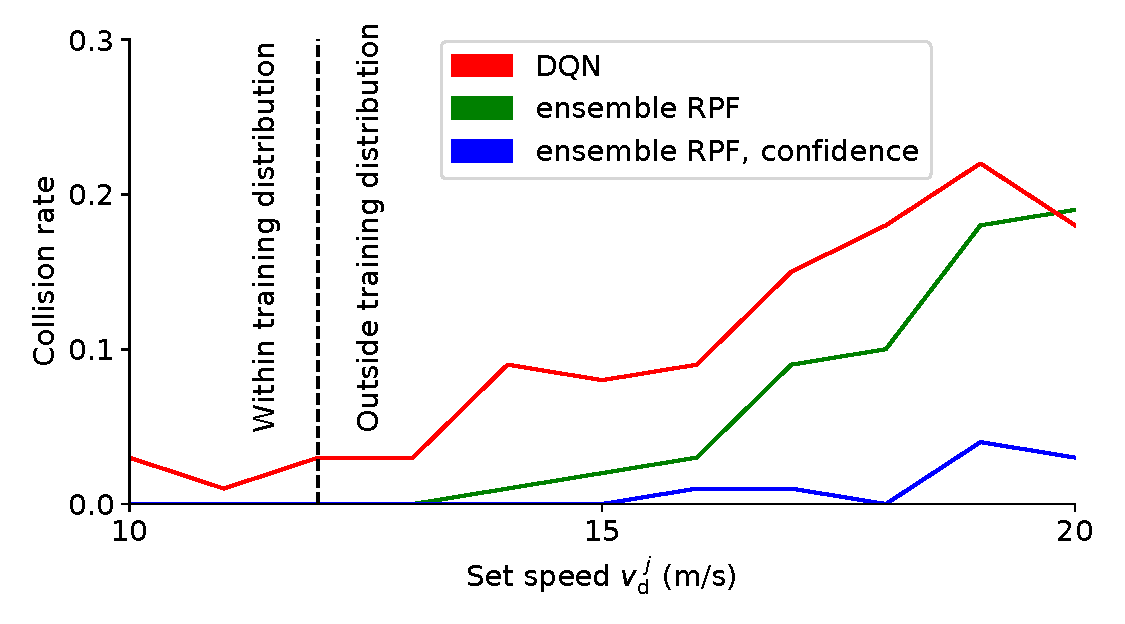
\includegraphics[width=0.99\columnwidth]{YourThesis/papers/ensamble/figures/collisions_outside_distribution_2_wo_type_3_fonts.pdf}
		\caption{Proportion of collisions.}
	\end{subfigure}
	
	\vspace{5pt}
	
	\begin{subfigure}[]{0.99\columnwidth}
	\centering
		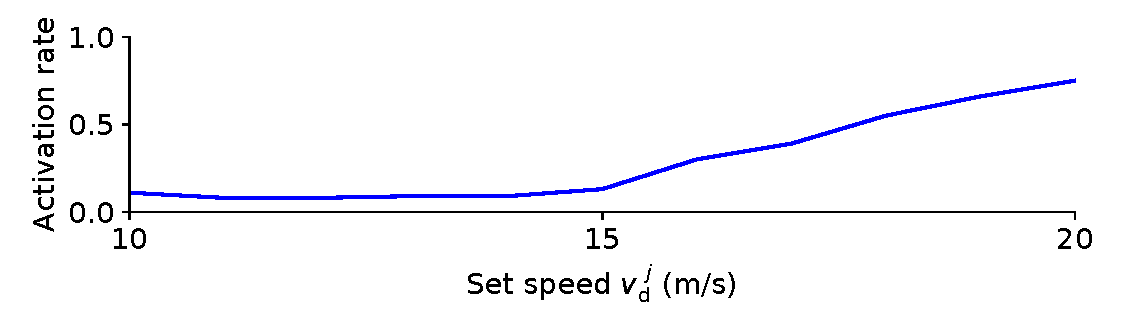
\includegraphics[width=0.99\columnwidth]{YourThesis/papers/ensamble/figures/activation_rate_2_wo_type_3_fonts.pdf}
		\caption{Proportion of episodes where $a_\mathrm{safe}$ was used at least once.}
	\end{subfigure}
	\caption{Performance of the ensemble RPF agent, with and without the confidence criterion, and the DQN agent, in test episodes with different set speeds $v_\mathrm{d}^j$ for the surrounding vehicles. %The shaded areas show the standard deviation for $5$ random seeds.
	}
	}}
	% \label{fig:performanceOutsideDistribution}
\end{figure}

\begin{figure}[!t]
	\mbox{\parbox{\textwidth}{
	\centering
	\begin{subfigure}[t]{0.48\columnwidth}
		\centering
		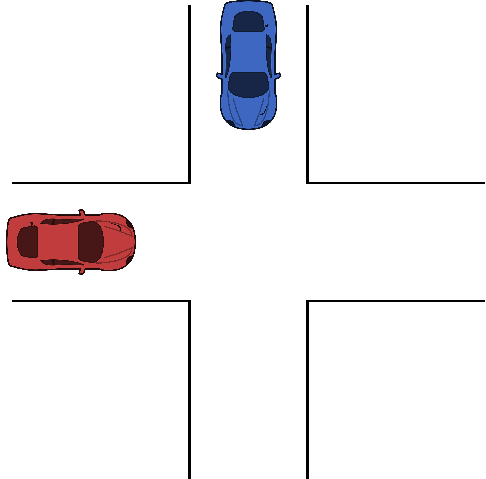
\includegraphics[width=0.7\columnwidth]{YourThesis/papers/ensamble/figures/figures-scen1.pdf}
		\caption{$t=0$, initial situation.}
	\end{subfigure}%
	~ 
	\begin{subfigure}[t]{0.48\columnwidth}
		\centering
		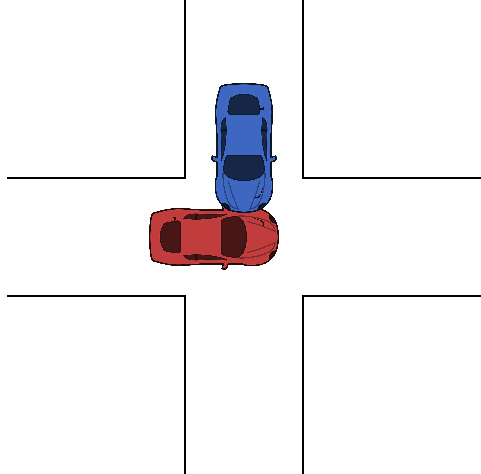
\includegraphics[width=0.7\columnwidth]{YourThesis/papers/ensamble/figures/figures-scen2.pdf}
		\caption{$t=1$, DQN and ensemble RPF without confidence criterion.}
	\end{subfigure}
	
	\vspace{5pt}
	
	\begin{subfigure}[t]{0.48\columnwidth}
		\centering
		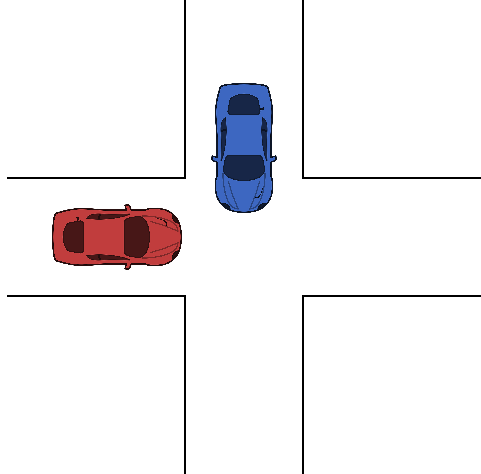
\includegraphics[width=0.7\columnwidth]{YourThesis/papers/ensamble/figures/figures-scen3.pdf}
		\caption{$t=1$, ensemble RPF with confidence criterion.}
	\end{subfigure}
	~ 
	\begin{subfigure}[t]{0.48\columnwidth}
		\centering
		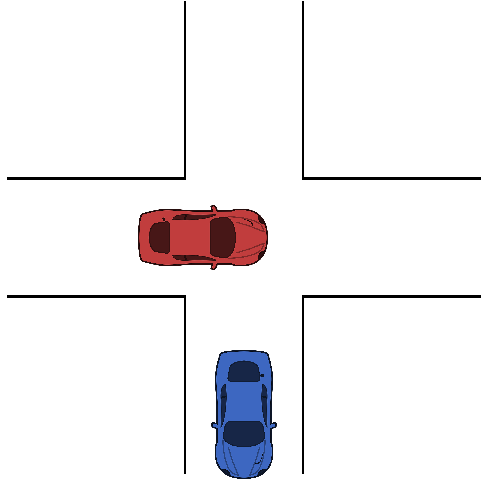
\includegraphics[width=0.7\columnwidth]{YourThesis/papers/ensamble/figures/figures-scen4.pdf}
		\caption{$t=1.5$, ensemble RPF with confidence criterion.}
	\end{subfigure}
	}}
	\caption{Example of a situation outside of the training distribution,
	where there would be a collision if the confidence criterion is not used. The vehicle at the top is here approaching the crossing at $20$ m/s.}
	% \label{fig:collisionOutsideDistribution}

\end{figure}

We show two approaches of handing uncertainty. with an estimate of the uncertainty in actions we showed that it can be used to reduce collisions and risk by choosing another policy than the one trained on data it is not confident in. 
The other work show how bad \gls{dqn} is at handing uncertainty in the input space. The results from the experiments show that the algorithms trained with an estimate from the probability distribution outperformed the algorithm trained with the probability distribution as inputs. 
\chapter{Generalizing over different scenarios}
\tommy{Uncertainty in MDP which one are we in?}
As mentioned in the Seciton \ref{sec:mdp}. The \gls{mdp} is defined by the tuple (S,A,R,T,$\gamma$). The work until now has solved the \gls{mdp} or \gls{pomdp} without defining the transition function T thanks to \gls{rl}. So what happens when you take a policy trained on one \gls{mdp} defined by one transition function? Well the short answer is that because \gls{dqn} uses a \gls{nn} to approximate the utility Q for taking an action in each state. 

Application areas. A transition function is defined as the probability of transitioning from one state to another. This could be different for example when the ego vehicle properties are different, if the DQN is trained on a sports car and then applied on a truck, the difference in acceleration capability would result in a different transition function. Another example would be on the other traffic participants, if the DQN is train in an environment where the driving culture is on the passive side and that is later put in an environment that has a more aggressive driving culture. The DQN/policy would probably not perform so well. 
This is especially important when you have an intention state directly correlated with the transition. For example in \paperD were the intentions are described on a high level such as take way or give way. 
An example is lane changes in Sweden, it is normal to signal first, wait for the other vehicle to slow down before initiating a lane change. While in a high density traffic jam in Paris, it is more normal to show intention by starting a lane change and observe if the other vehicle yields. 

\section{Approach}
Some easy solutions would to be have some geo identifier that can choose which policy to use given the country. That may work for an L4 system but could show to be difficult for an L5 system. Our approach is to use transfer RL to identify where we are in the convex hull of MDPs and then choose the policy for MDP we are closest too. 
This does require some number of MDPs to span out the convex hull of models. 
This can find a policy between MDPs. 
Identify which MDP is closest. For example Downtown driving in one country may be similar to the driving stile to another. 
\todo{cons: computationally heavy. Have to create the complex hull of MDPs from e set of MDPs.}
\todo{Pros: able to identify which policy to use and scale better by generalizing MDPs instead of countries.}


\section{Simulated experiments}
\section{Results and discussion}
FILL
\chapter{Discussion}
\label{ch:discussion}
Chapter 4, 5 and 6 introduce different methods to create a decision-making agent for navigating through intersections using deep Q-learning, while considering the uncertainty of its own decisions and the prediction of the other drivers intentions. This chapter highlights some differences and synergies of the different methods. 

\section{Guaranteeing safety}
\label{ch:system_architecture}
Safety is the most important factor of a \gls{ad} system, but since \gls{rl} is a data driven approach it is very difficult to guarantee safety in the same way e.g., a \gls{mpc} can. Safety validation in a data driven approach can be very costly as it is usually done by driving many miles and showing statistical confidence in the safety metrics~\cite{koopman2016,asljung2017}, e.g., number of interventions. That is why this section will clarify where the work in this thesis would fit in by first defining a system architecture for \gls{ad}, its modules and a short summary of the ISO 26262 standard. Then, place itself within the system and motivate how safety can be guarantied. 

The architecture of an autonomous driving system can be divided into perception, planning and control~\cite{Schwarting2018,Kortenkamp2008}.
The perception module is responsible for sensing and mapping the environment with the use of sensors such as LIDARs, cameras, radars etc. The raw data from the sensors are then processed though various sensor fusion techniques to generate a representation of the environment, e.g., position, velocity of other traffic participants while also describing the road such as width and distance to the next intersection. This information is then used by the planner to create a driving strategy of how to transverse through the world. However, the information from the sensors are often noisy, with false positives and false negatives making it difficult for the planner.

Tactical planning can be divided into three categories, the proactive, active and reactive~\cite{Berntorp2018}. A proactive module would be something like a precautionary safety module that interprets the information about the environment and create constraints that is sent to the active planner, like  driveable area, allowed speeds and actions~\cite{Shiller2007}. These constraints are generated from a set of safety goals and rules, making this the first layer of protection that can ensure safety. 
The role of the active planner is to take this sets of allowed actions and prescribe the behavior of the vehicle through decisions such as drive, yield or stop. The goal of these high level decisions is to optimize metrics such as comfort, fuel consumption and time to goal. These decisions are then sent to a motion planner that generates a safe dynamically feasible path for the vehicle for a shorter planning horizon of around $0.1$s. 
At the same time, a reactive, collision avoidance, module make sure that the chosen decision and path does lead to any collisions~\cite{brannstorm2010}. Unlike the decision maker, the collision avoidance module main goal is to identify imminent danger~\cite{brannstorm2014} and therefore has access to more aggressive actions like emergency braking to ensure safety. 
 
In the industry today the main standard for functional safety in motorized vehicles is the ISO 26262 standard, titled "Road vehicles – Functional safety"~\cite{ISO26262}. It uses a \gls{asil} to classify the inherent safety risk in an automotive system and the functions or modules of such a system. The \gls{asil} classification is used to express the level of risk reduction required to prevent a specific hazard, from \gls{asil} D to \gls{asil} A. \gls{asil} D represents the highest hazard level and \gls{asil} A the lowest. There is a level with no safety relevance and only standard Quality Management processes are required, this level is referred to as QM.

\begin{figure}[h]
	\centering
	%  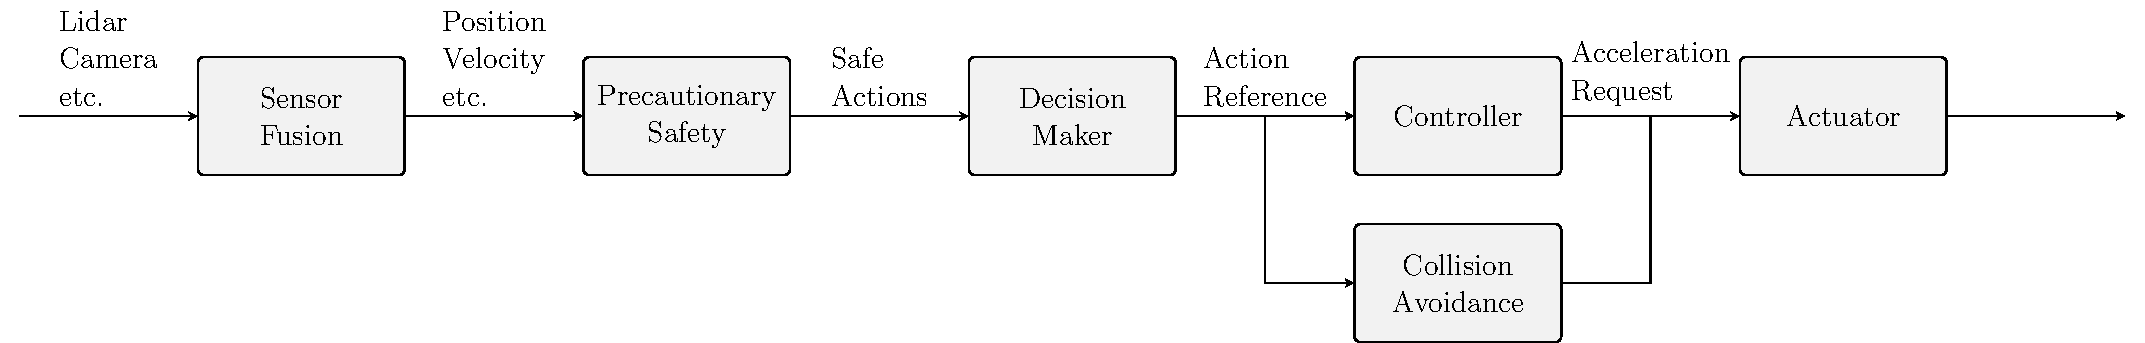
\includegraphics[width=\linewidth]{YourThesis/chapters/figures/pomdp/figures-system_architecture.pdf}
	\begin{tikzpicture}[
		node distance=8mm and 16mm,
		node font= \small,
		box/.style = {draw, thick, rectangle, rounded corners=0.1cm, fill=gray!10, minimum width=1.5cm, minimum height=1cm, align=center},
		% sx+/.style = {xshift = 1mm},
		sx+/.style = {xshift = 1mm}
		]
		
		\node (start1) at (0,0) {};
		\node[circle, draw, dashed, thick, fill=gray!30, minimum size=1.0cm] (world) {World};
		\node (SF) [box, right=of world.east] {Sensor \\ Fusion};
		\node (PS) [box, right=of SF.east] {Precautionary \\ Safety};
		\node (DM) [box, below=of PS.south] {Decision \\ Maker};
		\node (Con) [box, below=of SF] {Controller};
		\node (CA) [box, below=of Con] {Collision \\ Avoidance};
		\node (Act) [box, below=of world, yshift=.08cm] {Vehicle};
		\node (end) [left=of Act] {};

		\draw[->,thick,align=left] (world) --+(SF) node [midway,above] {Lidar\\Camera\\etc.};
		\draw[->,thick,align=left] (SF) --+(PS) node [midway,above] {Position\\Velocity\\etc.};
		\draw[->,thick,align=right] (PS) -| ($(PS.east) + (.5,0mm)$) |- (DM) node [above, xshift=10mm, yshift=5mm] {Safe\\Actions};
		\draw[->,thick,align=left] (Con) --+(Act) node [midway,above, xshift=3mm] {Acceleration\\Request};
		\draw[->,thick,align=left] (Act) -| ($(Act.west) - (.5,0mm)$) |- (world) node [midway,left] {};
		\draw[->,thick,align=left] (DM) --+(Con) node [midway,above] {Action\\Reference};
		\draw[->,thick,align=left] (DM) -| ($(DM.west) - (1,0mm)$) |- (CA) node [midway,above] {};
		\draw[->,thick,align=left] (CA) -| ($(CA.west) - (.7,0mm)$) |- (Act) node [midway,above] {};

	\end{tikzpicture} 
	\caption{Representation of the system architecture.}
	\label{fig:system_architecture}
\end{figure}

Although safety is the most important requirement for enabling autonomous driving, the work in this paper does not make any safety guarantees. Instead, it is proposed that the decision-making algorithms presented in this paper be used in the system architecture shown in Figure~\ref{fig:system_architecture}. This approach allows higher \gls{asil} to be applied to the precautionary safety and collision avoidance modules, while the decision-making algorithms focus primarily on comfort. As a result, the \gls{asil} classification for the decision-making components could be at lower levels, potentially even classified as QM in the best case.

\section{Designing the reward function and terminal states}
The reward function introduced in Chapter~\ref{ch:reward_function_def} is a crucial component that significantly influences the behavior and performance of a reinforcement learning agent. By carefully designing and tweaking the reward function in \eqref{eq:thesis_reward_function}, the agent can be guided towards desirable behaviors and optimize its decision-making policy. 

The results from Chapter~\ref*{ch:modeling_intersection} and \ref{ch:uncertainty} show a collision rate of $1-3\%$, which may seem high for \glspl{av}. However, within the proposed system architecture from Figure~\ref{fig:system_architecture}, this collision rate can be interpreted as interventions by a collision avoidance system, such as emergency braking. This interpretation can be achieved by adjusting the simulation parameters, for example, increasing the size of the cars or redefining the collision state to represent a collision avoidance intervention state.

% In comparison to \paperLSTM \ and \paperMPC, the need for a terminal state was removed for \paperEnsamble \ and \paperBelief, by excluding that state transaction in the experience replay, effectively allowing the agent to continue forever. While in \paperLSTM \ there was a negative reward for choosing an action to follow a non-existing car. This could also be removed by using Q-masking in \paperMPC \ and \paperEnsamble. 


\section{Modular models in autonomous vehicles}
There are two common strategies for creating and deploying \glspl{dqn} to the real world: training a comprehensive model that encapsulates everything or training smaller, specialized models and switching between them as needed. The proposed MLEMTRL algorithm from Chapter~\ref{ch:generalize} is a step towards the latter approach of using smaller models. Combined with the uncertainty measurements in Chapter~\ref{ch:uncertainty}, instead of reverting to a default action when uncertainty is high, the agent can instead trigger a model change. MLEMTRL can then be used to determine which model to switch to, ensuring a more adaptive and robust decision-making process.

This approach allows for modularity and flexibility, enabling easier updates and maintenance since individual models can be refined or replaced without affecting the entire system. Additionally, smaller models are less likely to overfit to irrelevant details present in a larger, comprehensive dataset, leading to more generalizable and robust performance in their specific domains. They also require less computational power and memory, making them more suitable for deployment on \gls{av}s with limited resources. Smaller models are generally easier to interpret and debug, facilitating understanding of the decision-making process and identifying any issues or biases, which is an important property to have when developing \gls{av}s.

% \section{Simulation and real world}
% Bridging the gap between simulation and real world. Ever evolving driving styles. Building trust. 
% Public trust is essential for the widespread adoption of AVs. Building this trust requires addressing concerns about safety, reliability, and the overall impact of AVs on society.
% Transparency and Communication: Providing clear and transparent information about how AV systems work, their safety features, and their limitations can help in building public trust. This includes communicating the results of safety tests and real-world performance data.
% Regulatory Compliance: Ensuring that AVs meet or exceed regulatory standards for safety and performance is crucial. Collaborating with regulatory bodies to establish and adhere to stringent safety protocols can reassure the public.
% Demonstrations and Pilot Programs: Conducting public demonstrations and pilot programs can help in showcasing the capabilities and safety of AVs. Allowing people to experience AVs firsthand can alleviate fears and misconceptions.
% !TEX root=../../Thesis.tex
\chapter{Concluding remarks and future work}
\section{Conclusions}\label{sec:conclusion}

1. RL by itself still has a long way to guarantee safety, but the methods presented in this paper. the unncertainty can be reduced. safety is better suited for contrl or formal methods. RL is a great tool for creating policy that can adapt to different driver interntions. 
2. Even with todays advancements in \gls{nn} DQN still has a hard time handling 
\section{Future work}
FILL

\includepapersummary % Label: 'chap:papersummary'. Replace with separate file if the auto-generated summary does not work with your content.

%==============================================================